\documentclass[11pt]{article}

\usepackage{deauthor}
\usepackage{times,graphicx}

% user packages
\usepackage{algorithm}
\usepackage{algorithmic}
\usepackage{float}
\usepackage{url}
\usepackage{todonotes}
\usepackage{subcaption}

\usepackage{pifont}
\usepackage{newtxtext}
\usepackage{newtxmath}
\usepackage{newclude}
\usepackage{multirow}
\usepackage{hyperref}
\usepackage{CJK}
\usepackage{cite}
\usepackage{booktabs}
\usepackage{balance}
\usepackage{caption}
\newcommand{\xmark}{\ding{55}}
\newcommand{\cmark}{\ding{51}}

\usepackage{graphicx}

\renewcommand{\dblfloatpagefraction}{.9}

% unnecessary commands

\usepackage{paralist}
\newcommand{\entity}{\mathcal{E}}
\newcommand{\relation}{\mathcal{R}}
\newcommand{\lang}{\mathcal{L}}
\newcommand{\model}{\mathcal{M}}
\newcommand{\term}{\mathcal{T}}
\newcommand{\kgnew}{\mathcal{KG}}

\title{QALinkPlus: Text Enrichment with Q\&A data}

% DONE:Email line is somehow too long
\author{ Yandong Sun
\hspace{2em}  Yixuan Tang \thanks{*Yixuan Tang and Anthony K.H. Tung are co-corresponding authors}
\hspace{2em}  Anthony K.H. Tung  \footnotemark[1]\\
%  School of Computing, National University of Singapore, Singapore\\ \parbox{0.9\textwidth}{\texttt{\small\{yandong,yixuan,atung\}@comp.nus.edu.sg}\\
% }
School of Computing, National University of Singapore, Singapore \\
\texttt{\small\{yandong,yixuan,atung\}@comp.nus.edu.sg}\\
}




\begin{document}

\maketitle

\begin{abstract}
Text enrichment, the task of augmenting textual content by incorporating supplementary information to bridge knowledge gaps and enhance reader engagement, is a critical aspect of information retrieval. This study focuses on leveraging question answering datasets, such as Natural Questions and SQuAD, which contain human-validated content from diverse domains as valuable knowledge sources. While QA datasets hold promise for addressing informational needs, existing approaches, like employing dense retrieval for text enrichment, often result in QA pairs that may lack relevance, diversity, or inherent interest. To address these challenges, our paper proposes a novel graph-based method for text enrichment using QA pairs. We construct an entity co-occurrence graph derived from QA datasets and derive context-QA-specific subgraphs. Through rule-based path analysis, we develop an interpretable scoring system to assess the relevance and engagement value of each QA pair. By intelligently re-ranking QA pairs with our scoring system, our method delivers enriched text that fills knowledge gaps and captivates readers, thus improving the overall reading experience. This framework is not only effective in text enrichment tasks, but it also offers advantages for personalization and personal data management.
\end{abstract}
% \input{./chapter1.introduction.tex}

\section{Introduction}
\label{sec:intro}
% This paragraph introduces the advancement of QA domain due to transformers and QA datasets. Meanwhile, it highlights the vast knowledge contained in these datasets which can be used in other tasks as well
% The QA domain has experienced remarkable progress, largely attributable to the capabilities of neural architectures, especially transformers like BERT\cite{DBLP:conf/naacl/DevlinCLT19}, GPT\cite{radford2018improving}, and T5\cite{raffel2020exploring}. These models have showcased impressive proficiency in QA tasks, significantly when tested on comprehensive datasets like SQuAD and Natural Questions. Meticulously curated, these datasets not only serve as benchmarks to assess the reading comprehension abilities of advanced models but also further solidify the pivotal role of transformers in pushing the frontiers of machine comprehension. Beyond testing and training, these datasets represent treasure troves of human-verified knowledge. Their depth and breadth signify their importance in the QA domain and also point to potential opportunities to leverage this wealth of information in various tasks.



% This paragraph should introduce the motivation for text enrichment and give an example to illustrate the challenges of applying the dense retrieval framework in text enrichment
% Motivation of the text enrichment task
% It should contain examples and motivation
As readers navigate vast expanses of textual content, they often come across areas where gaps in their knowledge surface or where they develop a curiosity about related topics. Question and Answer (QA) datasets, with their reservoir of knowledge, have the potential not only to bridge these knowledge gaps but also to enrich the text with related information that readers may find intriguing. Let's consider the novel "Harry Potter and the Philosopher's Stone" for an example. As shown in Fig\ref{fig:hp_example} (left), the novel contains various entities. An ideal set of QA pairs for this novel should explore these entities, ensuring that the questions and answers remain intimately connected to the novel's context. What's more, an ideal QA pair should delve deeper than surface-level details. A superficial question such as ``Who is the main character in this book?" with the answer ``Harry Potter" might emerge. This type of QA pairs effectively evaluates a QA model's comprehension of the book, but for a reader, the provided information, though accurate, might seem superficial, even if they are not deeply familiar with the story. 


% However, they aren't inherently designed to provide answers that are interesting, informative, and relevant to a specific context. 

% Issues of existing approaches
To effectively leverage QA pairs in augmenting textual content, the work QALink\cite{DBLP:conf/cikm/TangHLTWYZ17} first addressed and formulated the task of text enrichment. It designed a novel system to enhance the reading experience of text documents by automatically integrating relevant QA content from sites like Quora and StackExchange. This system aims to provide readers with supplementary information that aids in understanding and deepening their knowledge of the document's content. 

In the development of QALink, a neural network was trained to identify and retrieve relevant QA pairs, a task that has seen significant advancements with the advent of dense retrievers. These modern models are particularly adept at this retrieval task. However, applying dense retrievers directly for text enrichment can sometimes lead to a superficial engagement with the material. This is because they often highlight the most frequently mentioned entities, while overlooking the plethora of subtler details that are crucial for a thorough understanding of the text. For example, as shown in the right panel of Fig.\ref{fig:hp_example}, the introductory paragraph of the Harry Potter Wiki mentions numerous entities. Yet, a RoBERTa model trained on the Natural Questions dataset tends to focus the top 100 QA pairs predominantly around the most prominent entity, `Harry Potter', at the expense of less prominent ones. 

%This pattern of focusing on more common entities and neglecting rarer ones in dense retrievers is also observed in the study cited as \cite{sciavolino2021simple}. It highlights a key challenge: while dense retrievers perform exceptionally well with familiar entities, their efficacy diminishes when it comes to queries involving less common entities.

%This could be caused by the fact that dense retrieval models generalize poorly on rare entities.


% Highlight the challenges in an individual paragraph
When attempting to leverage a dense retrieval framework \cite{DBLP:conf/emnlp/KarpukhinOMLWEC20} directly for text enrichment, three challenges arise:
\begin{enumerate}
    \item \textbf{Lack of Diversity} Dense retrievers have a tendency to favor QA pairs concerning prevalent entities, resulting in a repetitive and predictable selection that overlooks the richness of less common entities and diminishes the breadth of exploration for the reader
    \item \textbf{Lack of Interestingness} The content surfaced by dense retrievers, while contextually accurate, often lacks the depth and engagement necessary to satisfy readers' curiosity or add meaningful insights to the text. In short, they are not interesting.
    \item \textbf{Irrelevant QA pairs} Despite their technical proficiency, dense retrievers occasionally present QA pairs that are not closely related to the text. These pairs, while possibly relevant in a broader context, fail to align with the specific themes, characters, or events in the narrative, leading to a disjointed enrichment experience for the reader.
    
    % \item \textbf{Unclear Connections} The relevance of certain QA pairs to the primary text can be obscure, presenting challenges in drawing clear connections that contribute to the reader's understanding and appreciation of the content.
\end{enumerate}

\begin{figure}[h]
  \centering
  \begin{minipage}{.5\textwidth}
    \centering
    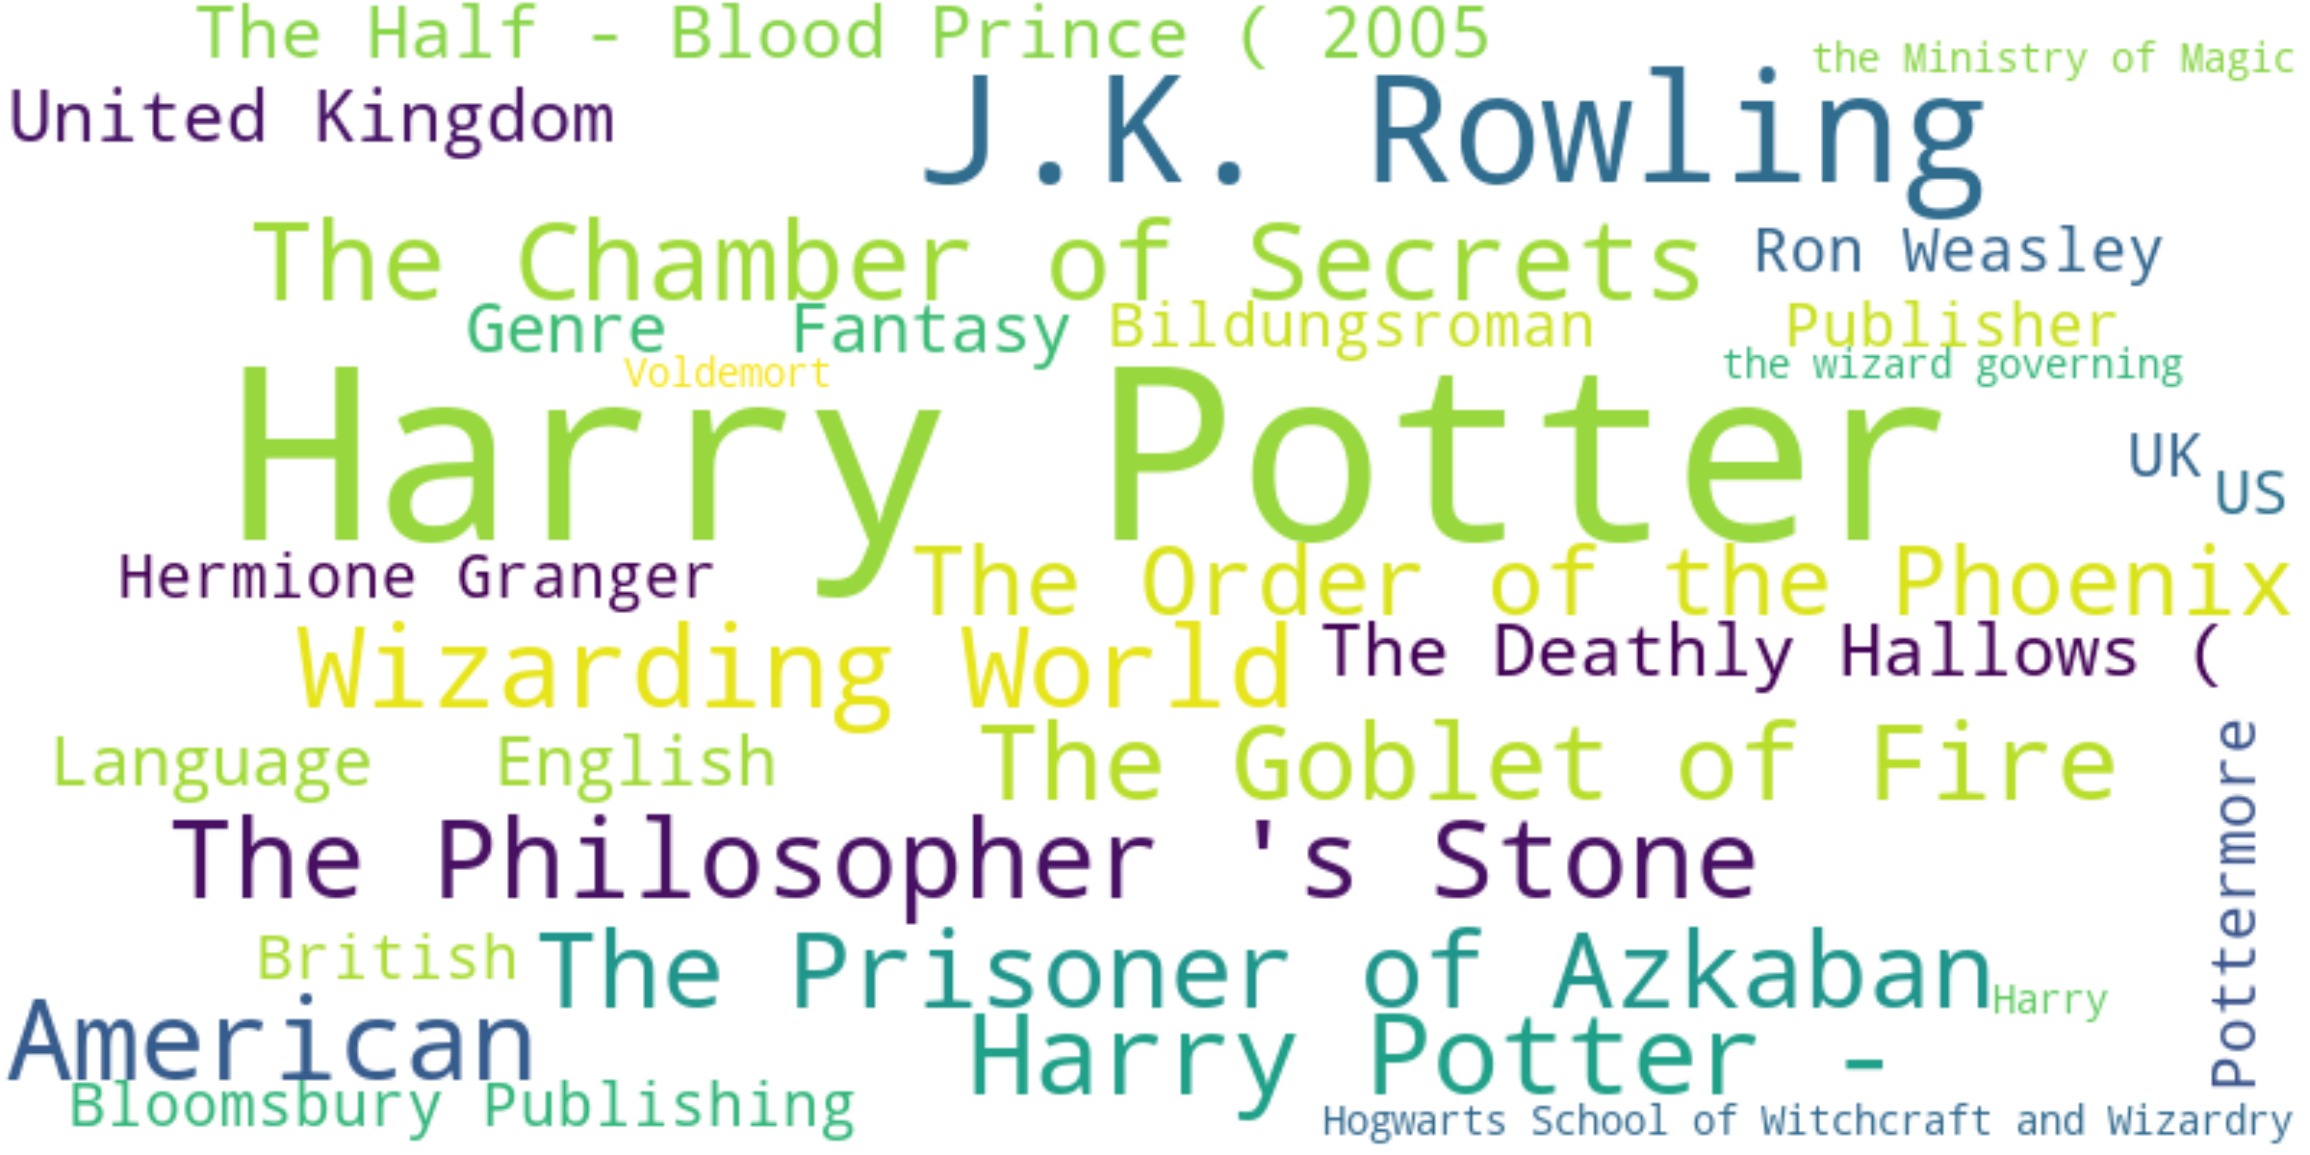
\includegraphics[width=.85\linewidth]{submissions/Tung2023/figs/hp_context_wordcloud.png}
    \label{fig:wordcloud1}
  \end{minipage}%
  \begin{minipage}{.5\textwidth}
    \centering
    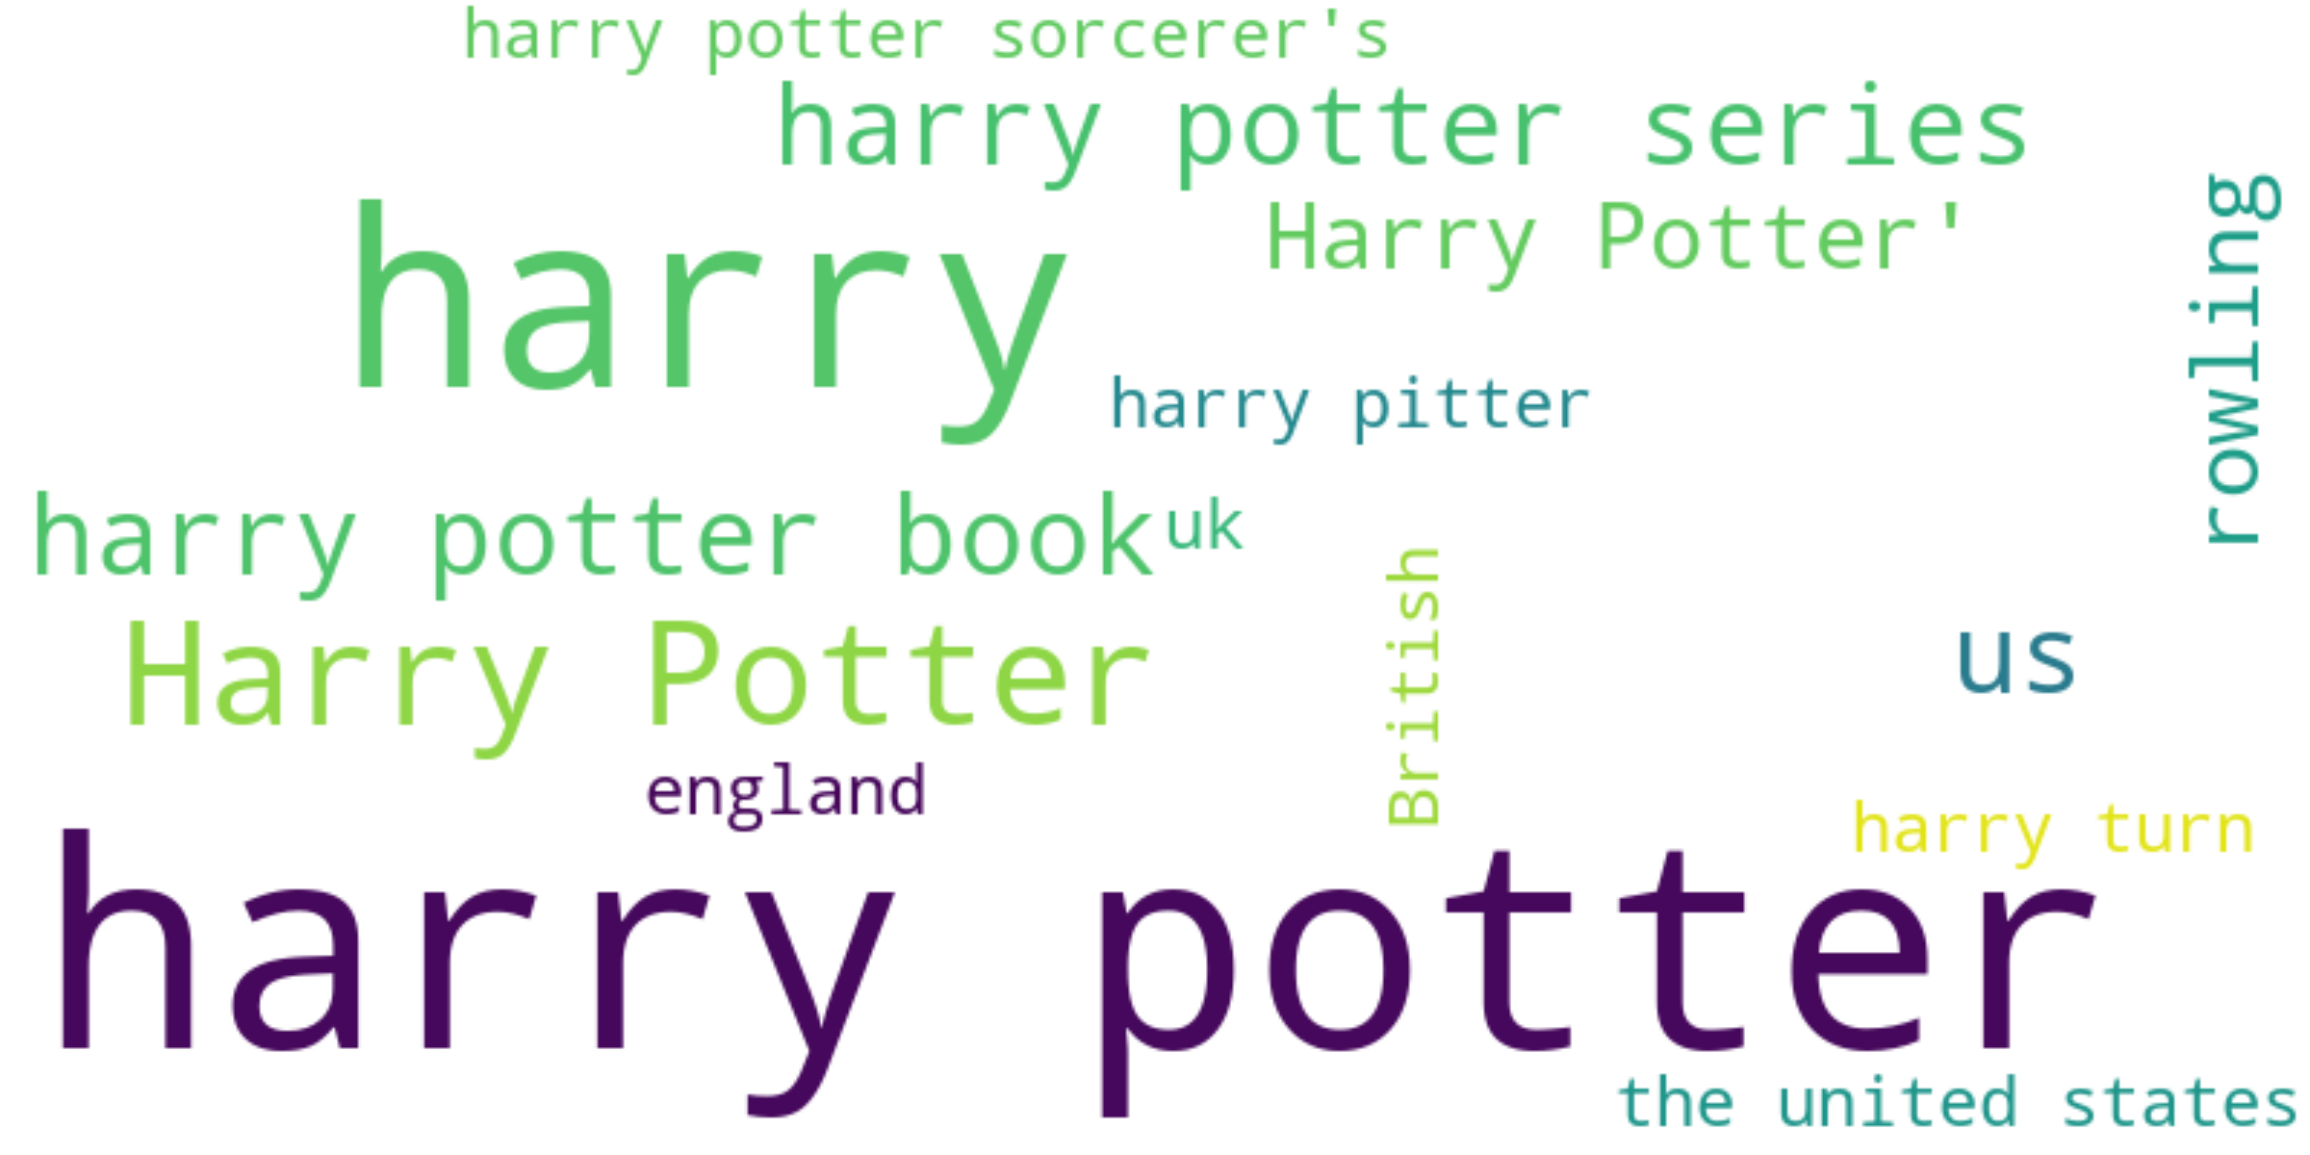
\includegraphics[width=.85\linewidth]{submissions/Tung2023/figs/hp_qa_wordcloud.png}
    \label{fig:wordcloud2}
  \end{minipage}
  \caption[Short Caption for LoF]{Comparison of the most frequently occurring named entities extracted. (Left) Entities derived from the introductory paragraph of the Harry Potter wiki page; (Right) Entities extracted from the top 100 QA pairs retrieved by querying the Harry Potter wiki content.}
  \label{fig:hp_example}
\end{figure}

% This paragraph should lead to the interestingness model
% Furthermore, the essence of "interesting" is somewhat elusive to dense retrieval models. While they can gauge relevance based on patterns seen during training, determining what is "interesting" to a human reader requires a level of subjectivity and intuition that these models don't inherently possess. It's also worth noting that dense retrieval models excel when the goal is clear-cut retrieval based on semantic similarity. However, when the task becomes multifaceted (ensuring relevance, depth, and reader interest), their default mechanisms might not suffice, necessitating more sophisticated or multi-pronged approaches.

% Introduce our framework
% TODO: Maybe need to provide a fig to illustrate our pipeline
% TODO: Entity Challenges also need to be mentioned
% TODO: Less use of the word 'psychology'
% TODO: References
% TODO: refine with recall

% [Purpose: Introduction and Conceptual Basis]
% To present an overview of the innovative approach, connecting it with psychological concepts of interestingness and outlining the proposed solution's novelty in addressing challenges in Q&A dataset enrichment.

% Our work confronts the challenge of enhancing text with QA datasets through a unique method that combines conceptual psychological model of interestingness with computational techniques. Taking cues from psychological theories that identify novelty and complexity as key drivers of interest, we apply these concepts to the realm of text enrichment. Our approach begins with constructing an entity co-occurrence graph from QA datasets, setting the stage for a deeper, more contextual analysis. By doing so, we bring a traditionally theoretical understanding of engagement into a practical, computable framework, paving the way for enriched text that is both informative and intriguing to readers.

%[Purpose: Methodological Detail]
% To describe the specific methodology, detailing the construction of the entity co-occurrence graph, subgraph extraction, and the application of rule-based path analysis informed by the psychological model of interestingness.

% Move this part into Mehodology
% Diving deeper into our method, we elaborate on the construction of an extensive entity co-occurrence graph from QA datasets, which underpins our technique. Entities within the context and corresponding QA pairs are mapped onto this graph to extract relevant subgraphs. Informed by the psychological constructs of novelty and complexity, our rule-based path analysis navigates these subgraphs. This meticulous scrutiny not only engenders an interpretable scoring system but also clarifies the connections between context and QA pairs, which may not be immediately evident to readers. This approach empowers a more nuanced and compelling enrichment of text, elevating the reader's interaction with the content.

%[Purpose: Outcomes and Advancements]
%To highlight the outcomes of applying the methodology, focusing on how it advances beyond traditional psychological models and provides a computable solution that elevates the reading experience through engaging, relevant text enrichment.
% Applying this innovative framework enables us to refine the selection of QA pairs, foregrounding those that are not only pertinent but also inherently intriguing to the reader. This enhances the reading experience by ensuring the text is engaging and informative. Our advancement over traditional psychological models is significant; we not only delineate the theoretical aspects of what makes content interesting but also translate these theories into a practical, algorithmic format. The resultant model is not a mere theoretical construct but a dynamic, computable system that captures the essence of interestingness and applies it to text enrichment, thereby bridging the gap between abstract psychological concepts and their tangible, computational applications.

% In the last paragraph, the personalization and privacy need to be mentioned as well
Our work confronts the challenge of enhancing text with QA datasets through a unique method. We construct an extensive entity co-occurrence graph from QA datasets, crucial for our text enrichment technique. We map entities from the text and corresponding QA pairs onto this graph to identify relevant subgraphs. Through rule-based path analysis, influenced by the psychological principles of novelty and complexity, we not only develop an interpretable scoring system but also unveil the nuanced connections between context and QA pairs. This approach enriches the text in a nuanced and engaging manner. By refining QA pair selection, our method ensures relevance and diversity while captivating the reader's interest at the same time. This advancement goes beyond traditional models, applying psychological theories of content interestingness in a practical, algorithmic way. Our framework stands out as a system that intertwines psychological concepts with computational applications, enhancing the reading experience by making it more engaging and informative. What's more, we have also discussed how our framework can be used in personal data management and personalization in Sec.\ref{Pesonalization}.

% \begin{figure}[h]
%     \centering
%     \includegraphics[width=0.5\linewidth]{submissions/knowledge-sentiment-analysis/2.png}
%     \caption{Sentences with different contexts or based on external common sense knowledge can express different sentiments. Expressions carrying positive (smiling face) or negative (crying face) sentiments are highlighted in color. }
%     \label{fig:Example}
% \end{figure}

The main contributions of this paper can be summarized as follows:
\begin{itemize}
    \item \textbf{Modeling Interestingness Through Psychology Principles:} We propose a model that assesses interestingness by considering both novelty and complexity, drawing inspiration from psychological research. This approach aims to provide a more nuanced understanding of what makes content engaging.
    \item \textbf{Entity Subgraphs for Context and QA Pair Representation:} Our method utilizes entity subgraphs as a simple yet effective way to represent context and question-answer pairs. We then employ path analysis to evaluate the interestingness of these contexts and QA pairs, offering an interpretable and efficient mechanism for analysis.
    \item \textbf{Optimization for Enhanced Contextual Coverage in QA Pairs:} We've formulated an optimization problem aimed at maximizing the coverage of context entities in the QA pairs retrieved and proposed a near-optimal solution that is both practical and efficient. This serves as a re-ranking strategy post-dense retrieval. This approach specifically addresses the challenge of forming robust representations for frequent entities, while also enhancing the distinction of less common ones in text enrichment tasks.
\end{itemize}

% \input{./chapter2.relatedwork.tex}
\section{Related Work}

% May need to change this title. Changed.
% Less words about interestingness here.
% This series of works are to highlight our contribution and novelty
% \paragraph{\textbf{Interestingness}} The exploration of 'interestingness' in computer science has led to the categorization of captivating objects under various terms such as 'Fun Facts' \cite{DBLP:conf/wsdm/TsurelPGS17}, 'Semantic Novelty' \cite{DBLP:conf/emnlp/MaPMC00G21}, 'Trivia' \cite{DBLP:conf/aaai/FatmaCS17}\cite{DBLP:conf/ijcai/PrakashCPG15}, and 'Unusual Aspects' \cite{DBLP:conf/aaai/FatmaCS17}. Numerous studies have delved into the concept of 'interestingness' \cite{DBLP:conf/eacl/KamigaitoKSO21}\cite{DBLP:conf/ijcai/PrakashCPG15}\cite{DBLP:conf/aaai/FatmaCS17}, frequently emphasizing the role of rarity as a fundamental characteristic of what makes an object interesting. This perspective is notably articulated in \cite{DBLP:conf/aaai/FatmaCS17}, where the appeal of trivia is linked to its \textit{unusualness}, \textit{uniqueness}, or \textit{unexpectedness}, underscoring the idea that deviation from the norm is a key element of interest. However, this emphasis on rarity as the sole determinant of interestingness is somewhat limited. Rarity in itself may not always equate to interestingness; many rare objects are merely unpopular, thus not generally perceived as interesting. This observation raises a compelling question: what factors, in addition to rarity, contribute to an object's perception as interesting? While this inquiry might initially appear tangential to the core interests of computer science, the concept of 'interestingness' has been extensively explored in other disciplines, particularly psychology. Psychological research, dating back to at least 1910 \cite{bolton1910attention}, offers a distinct perspective from that of computer science. Studies by \cite{hunt1963affect}, \cite{fredrickson1998good}, and \cite{izard2000motivational} suggest that interestingness is intertwined with curiosity, exploration, and information seeking. Additional models explaining interestingness in various contexts have been proposed, such as those by \cite{schraw2001situational} and \cite{krapp1999interest}. These models, derived from human studies on abstract concepts and emotions, are challenging to quantify and render computable, which explains their limited appeal to computer science researchers. Despite this, the ongoing research into interestingness has highlighted the influence of novelty and complexity on this concept, as evidenced in the works of \cite{berlyne1960conflict}, \cite{berlyne1974studies}, and \cite{silvia2005interesting}. This relationship has been validated across various stimuli and measures of interest \cite{silvia2005interesting}. Unlike other abstract feelings and concepts, novelty and complexity are more amenable to mathematical modeling, as demonstrated by existing research on novelty. Therefore, we have identified complexity as an important aspect to further explore in our efforts to understand and quantify interestingness, particularly in the context of text enrichment tasks. This exploration aims to enhance our ability to measure and apply the concept of interestingness in computational analysis, enriching the textual content with elements that are not just rare, but genuinely engaging and thought-provoking. 



\paragraph{\textbf{Interestingness}}The concept of `interestingness' in computer science encompasses various captivating objects termed as `Fun Facts', `Semantic Novelty', `Trivia', and `Unusual Aspects', with many studies highlighting rarity as a key element \cite{DBLP:conf/wsdm/TsurelPGS17,DBLP:conf/emnlp/MaPMC00G21,DBLP:conf/aaai/FatmaCS17,DBLP:conf/ijcai/PrakashCPG15}. However, rarity alone doesn't always equate to interestingness, as some rare objects may simply be unpopular. This notion leads to the broader question of what additional factors make an object interesting. Psychological research offers insights into this, linking interestingness with curiosity, exploration, and information seeking \cite{bolton1910attention,tomkins1962affect,fredrickson1998good,izard2000motivational,schraw2001situational,krapp1999interest}. Current research in computer science, drawing from these psychological models, focuses on novelty and complexity as quantifiable attributes of interestingness \cite{berlyne1960conflict,berlyne1974studies,silvia2005interesting}. Recognizing this, our study emphasizes complexity alongside rarity in understanding and quantifying interestingness for text enrichment tasks, aiming to enrich textual content with elements that are not just rare but also genuinely engaging and thought-provoking.

% This series of works are to illustrate the challenges and limitations of current works
% \paragraph{\textbf{Dense Retrieval}} Dense retrieval is a crucial component in our text enrichment approach, especially due to its high recall in QA dataset applications, ensuring a strong relevance between context and QA pairs. This high recall is vital for enriching the context with relevant and informative QA pairs. Techniques like iterative passage retrieval, as proposed by \cite{DBLP:conf/iclr/DasDZM19}, and the encoding of candidate answer phrases as vectors for efficient retrieval, as in \cite{DBLP:journals/corr/abs-1906-05807}, exemplify the precision and efficiency of dense retrieval. These methods ensure contextually aligned and content-rich text enrichment. Additionally, dense retrieval is adaptable in scenarios lacking direct answers, such as retrieving supporting documents from sources like Wikipedia before answer extraction, as suggested by \cite{DBLP:conf/acl/ChenFWB17}. In situations without gold standard answers, techniques like global normalization over potential answer spans, as per \cite{DBLP:conf/acl/GardnerC18}, are invaluable for covering a wide range of possible answers, thereby enhancing the informational breadth of the text. The integration of these retrieval methods into our process not only maintains contextual relevance but also enriches the content with informative QA pairs, elevating the overall value and engagement of the enriched text. Despite their impressive performance within familiar domains, dense retrieval models exhibit limitations in generalizing to novel, unseen questions. Recent findings in \cite{DBLP:conf/eacl/LewisSR21} highlight a significant overlap between training and testing sets in popular QA benchmarks. This suggests that these models may tend to memorize training questions, leading to subpar performance on distinct, non-overlapping questions. Furthermore, AmbER\cite{chen2021evaluating} tests aimed at examining entity disambiguation capabilities of passage retrievers and entity linkers reveal a pronounced performance decline for models when dealing with rare entities compared to common ones. A critical study titled "Simple Entity-Centric Questions Challenge Dense Retrievers"\cite{sciavolino2021simple} sheds light on this issue, demonstrating that the Dense Passage Retriever (DPR) notably underperforms compared to BM25\cite{robertson2009probabilistic} on EntityQuestions — a dataset derived from Wikidata facts focusing on straightforward questions. This underperformance is primarily attributed to DPR's tendency to form robust representations for frequent entities, while struggling to distinguish less common ones without specific training on their associated question patterns. The crux of the issue lies in the fact that dense retrieval models, while effective in certain contexts, generally show poor generalization capabilities, particularly in identifying and differentiating rare entities. This not only impedes their utility in diverse real-world scenarios but also highlights a critical gap in their ability to cater to a wider range of informational needs — a gap our research aims to bridge by proposing a more nuanced, graph-based approach to question and entity evaluation. Our methodology intends to enhance the measurement of 'interestingness' in questions, factoring in the novelty, complexity, and contextual relevance that current models often overlook.

\paragraph{Related Text Retrieval} This series of research works involves finding relevant information or text passages based on a given query or input text. The variation of it that most related to our work is dense passage retrieval, the goal is to retrieve relevant documents or passages using dense vector representations of the texts. As proposed by \cite{DBLP:conf/iclr/DasDZM19}, and the encoding of candidate answer phrases as vectors for efficient retrieval, as in \cite{DBLP:journals/corr/abs-1906-05807}, exemplify the precision and efficiency of dense retrieval. These methods ensure contextually aligned and content-rich text enrichment. Additionally, dense retrieval is adaptable in scenarios lacking direct answers, such as retrieving supporting documents from sources like Wikipedia before answer extraction, as suggested by \cite{DBLP:conf/acl/ChenFWB17}. In situations without gold standard answers, techniques like global normalization over potential answer spans, as per \cite{DBLP:conf/acl/GardnerC18}, are invaluable for covering a wide range of possible answers, thereby enhancing the informational breadth of the text. However, the direct application of dense retrievers in text enrichment can lead to a superficial engagement with the content. This occurs because these retrievers tend to focus on the most commonly mentioned entities, thereby overlooking many finer details crucial for a comprehensive understanding of the text. This inclination towards prominent entities over subtler details, as noted in \cite{sciavolino2021simple}, highlights a significant challenge in employing dense retrievers for nuanced text analysis.

% This is mainly related to graph mining and why we do not use KG here.
\paragraph{\textbf{Question and Answer Datasets}}
% The question-answering (QA) domain has seen a significant evolution, largely driven by the development of diverse datasets such as SQuAD\cite{DBLP:conf/emnlp/RajpurkarZLL16}, Natural Questions\cite{DBLP:conf/eacl/KamigaitoKSO21}, TriviaQA\cite{DBLP:conf/acl/JoshiCWZ17}, and NarrativeQA\cite{DBLP:journals/tacl/KociskySBDHMG18}. These datasets, originally designed as benchmarks for evaluating reading comprehension in QA systems, have emerged as much more than mere tools for assessment. They are vast repositories of human-verified, structured knowledge, encompassing a wide array of topics and question-answer formats. This richness makes them particularly valuable for applications beyond their initial scope, such as text enrichment. In text enrichment tasks, the objective is to enhance the informational depth and contextual relevance of textual content. The varied nature of QA datasets, with their extensive collection of real-world questions and corresponding answers, provides a unique opportunity to extract and integrate nuanced contextual and factual information into text-based applications. This approach can significantly enrich the content, making it more informative, engaging, and valuable for end-users. Leveraging these datasets for text enrichment represents an innovative repurposing of their potential, moving beyond traditional QA challenges. It opens new avenues for exploiting the depth of QA datasets, transforming them into tools for enhancing the quality and richness of textual information in various domains, thereby contributing to the advancement of natural language processing and information retrieval techniques.


The evolution of the question-answering (QA) domain has been significantly influenced by the development of datasets like SQuAD\cite{DBLP:conf/emnlp/RajpurkarZLL16}, Natural Questions\cite{DBLP:conf/eacl/KamigaitoKSO21}, TriviaQA\cite{DBLP:conf/acl/JoshiCWZ17}, and NarrativeQA\cite{DBLP:journals/tacl/KociskySBDHMG18}. Initially created as benchmarks for QA systems' reading comprehension, these datasets have become much more than assessment tools. They are now vast repositories of verified knowledge across diverse topics and formats, making them ideal for applications such as text enrichment. In text enrichment, the goal is to deepen the informational and contextual quality of textual content. The varied and real-world questions and answers in these QA datasets offer a unique resource for embedding detailed contextual and factual information into texts, enhancing their informativeness and engagement for users. This re-purposing of QA datasets for text enrichment not only extends their use beyond traditional QA but also opens new paths in natural language processing and information retrieval, enhancing the quality and richness of textual content across various domains.


% \input{./chapter3.methodology.tex}
\section{Methodology}
\label{sec:methodology}
\subsection{Overview}
\begin{figure}[t]
  \centering
  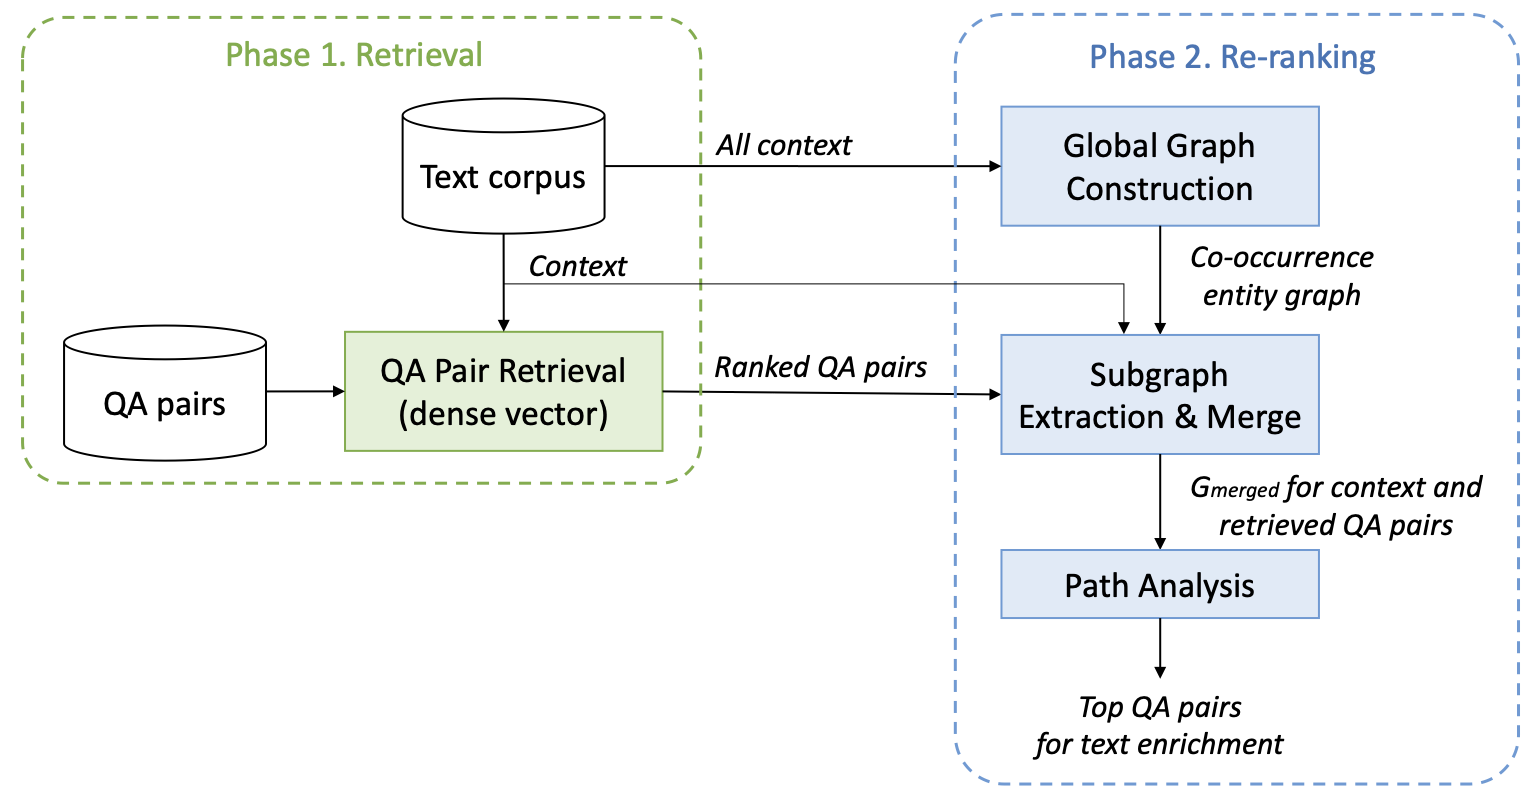
\includegraphics[width=0.8\textwidth]{submissions/Tung2023/figs/overview_1.png}
  \caption{Framework Overview}
  \label{fig:overview_1}
\end{figure}

Our framework operates as follows. Initially, we apply Named Entity Recognition (NER) to both a set of contexts (documents) and a set of QA pairs. From the contexts, we extract entities to build an entity co-occurrence graph, linking entities that appear within three sentences of each other. For any given context, we use its entities to identify a corresponding subgraph in this co-occurrence graph. The same process applies to a list of QA candidates. We then merge the subgraphs of each context and its respective QA pair into a unified subgraph. A path analysis is conducted on this united subgraph, using specially designed path patterns that assess novelty and relatedness, yielding an interpretable score. This score is used to re-rank the QA candidates. Additionally, to ensure the diversity of selected QAs, we optimize the QA candidates to maximize the coverage of linked context entities in the QA pairs, with each entity weighted according to its score from the path analysis step. This methodological approach facilitates a nuanced selection of QA pairs that are not only relevant but also diverse, enhancing the overall quality and informativeness of the enriched text. As shown in Fig.\ref{fig:overview_1}.




\subsection{Problem Formulation}
% Start with an introductory paragraph setting the stage. 
% Start with text enrichment first
%Advancements in QA systems have been noteworthy, especially with the development of sophisticated neural models and the curation of rich datasets such as Natural Questions and SQuAD. Yet, in the practical application of dense retrieval frameworks aimed at enriching textual interactions, the QA pairs often fall short in providing depth and relevance, resulting in an engagement that can be either mundane or contextually ambiguous for the reader.

% Detailed Statement of the Problem


% Research Gap
%At the heart of the problem, dense retrieval models exhibit limited generalization capabilities, particularly in identifying and distinguishing rare entities. This limitation not only hinders their effectiveness in varied real-world scenarios but also underscores a significant research gap in fulfilling diverse informational needs. Our research proposes a graph-based methodology aimed at addressing this gap. The focal point of our approach is enhancing the measurement of 'interestingness' in questions, which involves considering aspects such as novelty, complexity, and contextual relevance — elements often neglected by current models.

%Recognizing these limitations, our research pivots towards a novel approach that not only gauges the relatedness of questions to the textual content but also assesses their 'interestingness'. This shift in focus addresses the critical need for enriching reader experience with content that is not just contextually aligned but also intellectually stimulating and engaging. We propose a graph-based method paired with an 'interestingness' model, aiming to dynamically evaluate and suggest questions that not only connect with the text but also add depth and intrigue to the reader's exploration. This approach seeks to fill the gap in current dense retrieval frameworks, offering a more nuanced and engaging way to interact with and enrich textual content.

% Problem Formulation
% Our goal is to develop a system that can evaluate the "interestingness" of questions in a given context (like a text or a novel), using an entity graph to represent the context and the questions. The "interestingness" of a question will be gauged through its complexity, novelty, and the degree of its relatedness to the context.

% Advancements in QA systems, particularly with sophisticated neural models and datasets like Natural Questions and SQuAD, have been significant. However, when it comes to applying dense retrieval frameworks for text enrichment, these systems often provide QA pairs that lack depth and relevance, leading to mundane or contextually ambiguous reader engagement. At the core, these models struggle with generalizing, especially in identifying rare entities, highlighting a critical research gap in meeting diverse informational needs. Our research addresses this by proposing a novel graph-based methodology that focuses on the 'interestingness' of questions, factoring in novelty, complexity, and contextual relevance — aspects often overlooked by current models. This approach aims to enrich the reader experience with intellectually stimulating and contextually relevant content, filling the gap in existing dense retrieval frameworks and offering a more nuanced way to enhance textual interactions.

% We consider the task of text enrichment via QA datasets as a retrieval problem, and it will be introduced first.
 
% \paragraph{Formulation of Dense Retrieval for Text Enrichment} \textit{Given a context \( \mathcal{C} \) and a QA dataset \( \mathcal{D} = \{(q_1, a_1), \allowbreak (q_2, a_2), \allowbreak \ldots, \allowbreak (q_m, a_m)\} \), the goal is to train an embedding function \( \phi: \mathcal{X} \rightarrow \mathbb{R}^d \) that maps any textual content \( \mathcal{X} \) to a \( d \)-dimensional vector space such that the embeddings of contextually relevant QA pairs from \( \mathcal{D} \) are closer to the embedding of \( \mathcal{C} \), as determined by a similarity function \( \text{sim}: \mathbb{R}^d \times \mathbb{R}^d \rightarrow \mathbb{R} \). The objective is to maximize the relevance of the top \( k \) retrieved QA pairs for any given context \( \mathcal{C} \), which we formalize as the following optimization problem:}



% \begin{equation}
% \label{eq_1}
% \max_{\phi, \text{sim}} \sum_{i=1}^{k} \text{sim}(\phi(\mathcal{C}), \phi(q_i, a_i))
% \end{equation}

% The objective function defined \eqref{eq_1} seeks to maximize the aggregate similarity across the top \( k \) question-answer (QA) pairs from dataset \( \mathcal{D} \) that are most similar to the context \( \mathcal{C} \). Specifically, it sums the similarity scores between the context embedding \( \phi(\mathcal{C}) \) and the embeddings of the QA pairs \( \phi(q_i, a_i) \), selecting the pairs that contribute to the highest total similarity. This formulation implicitly performs a ranking by prioritizing the selection of QA pairs that have the greatest similarity to the given context, thereby obviating the need for an explicit ranking mechanism within the optimization function itself.

% Our approach proposes a nuanced, graph-based methodology for the evaluation of questions in terms of their 'interestingness', which we define based on their novelty, complexity, and contextual relevance. This model aims to address the current gaps in understanding and processing complex, novel, and contextually rich questions that standard dense retrieval models often fail to recognize or value appropriately.

Building upon the advancements in dense retrieval, our work introduces a nuanced problem formulation that explicitly captures both the `interestingness' and `relatedness' of QA pairs in relation to a given context. This dual consideration aims to enrich the textual landscape with engaging and pertinent information that transcends mere relevance, bringing to light the subtler aspects of human-like engagement and curiosity-driven exploration.


\textit{Our proposed problem formulation extends beyond the traditional objective of maximizing relevance. It introduces a composite measure that encompasses both the relatedness of QA pairs to the given context \( \mathcal{C} \) and the intrinsic interestingness of the questions \( q_i \) and answers \( a_i \) in the dataset \( \mathcal{D} \). The function \( \phi: \mathcal{X} \rightarrow \mathbb{R}^d \) remains central in embedding textual content into a d-dimensional vector space, while the similarity function \( \text{sim}: \mathbb{R}^d \times \mathbb{R}^d \rightarrow \mathbb{R} \) is now complemented by an interestingness function \( \text{int}: \mathcal{Q} \times \mathcal{A} \rightarrow \mathbb{R} \), which assesses the compelling nature of QA pairs. The combined optimization problem is then:}


\begin{equation}
\label{eq_interest_relatedness}
\max_{\phi, int} \sum_{i=1}^{k} ( sim(\phi(\mathcal{C}), \phi(q_i, a_i)), int(C, q_i, a_i ))
\end{equation}

% \begin{equation}
% \label{eq_general_problem}
% R' = \underset{q_i, a_i \in R}{\mathrm{sort}}\ \left[ \text{Relatedness}(\mathcal{C}, q_i, a_i) + \text{Interestingness}(q_i, a_i) \right]
% \end{equation}

% Here, the parameter \( \lambda \) serves to adjust the balance between interestingness and relatedness within the retrieval process. The objective function, presented in Equation~\ref{eq_interest_relatedness}, aims to optimize a composite score that concurrently evaluates the relevance and the engaging nature of the QA pairs. This ensures that the selected top \( k \) pairs are not only germane to the given context but also possess an intrinsic appeal that is likely to engage the reader. The 'interestingness' of the QA pairs is assessed through a dedicated function, hereinafter referred to as \( \textit{int} \).


% Given a list of question-answer pairs in \eqref{eq_1}, we introduce a re-ranking function that prioritizes interestingness. The re-ranking is achieved by sorting the QA pairs according to their interestingness scores. Formally, the re-ranking function $rerank$ can be defined as:

% \begin{equation}
% \label{eq_re-rank}
% R' = rerank(R) = \underset{q_i, a_i \in R}{\mathrm{sort}}\ int(q_i, a_i)
% \end{equation}

% Here, \( R \) is the set of retrieved QA pairs, and \( R' \) is the set after re-ranking, where $int(q_i, a_i)$ is the interestingness score for the $i $-th QA pair. The function \( \text{rerank} \) is designed to prioritize QA pairs with higher interestingness scores, thereby improving the overall engagement of the retrieved information.

In defining the interestingness of a question-answer pair within a given context, we draw upon two fundamental psychological constructs: novelty and complexity. Novelty (\textit{novelty}) reflects the degree to which information is new or surprising to a user, while complexity (\textit{complexity}) represents the intricacy and depth of the information presented. 

Our interestingness function, denoted conceptually as \(\text{Interestingness}(C,(q_i, a_i))\), thus incorporates both novelty and complexity. This conceptual function is not directly quantifiable but serves as a theoretical framework guiding the development of our computational model:

\begin{equation}
int(C,q_i, a_i) \propto \text{Novelty}(C,q_i, a_i) \oplus \text{Complexity}(C,q_i, a_i)
\end{equation}

Here, \(\oplus\) denotes a conceptual combination of novelty and complexity, the specifics of which will be operationalized in the subsequent computational model. This formulation underscores the importance of both elements in constituting what makes a question-answer pair engaging to the user.





\subsection{Proposed Methods}
% We need some transition or an overview of our method here. And a fig to show the overview of framework.

\subsubsection{QA-pairs Retrieval}
Drawing inspiration from the remarkable success of dense retrievers in passage retrieval tasks, as highlighted in \cite{DBLP:conf/acl/ChenFWB17}, we have adopted this framework to retrieve relevant question-and-answer (QA) pairs for a given context. Specifically, we employ the RoBERTa-base model, which has been fine-tuned on the Natural Questions dataset using a contrastive learning approach. In this approach, positive and negative examples are constructed with a focus on the relationship between context and QA pairs. For a batch size of \( N \), positive examples are \( N \) pairs such as \((C_1, q_1, a_1), (C_2, q_2, a_2), \ldots, (C_N, q_N, a_N)\), where each \( C_i \) represents a context and \( q_i, a_i \) its corresponding question and answer. Negative examples are generated by mismatching the contexts and QAs, pairing different \( C_i \) with \( q_j, a_j \) where \( i \neq j \). The loss function is NT-Xtent as Eq.\ref{eq:loss_func}, where $\tau$ is the temperature parameter that helps to control the scale of the similarity scores. This method enhances the model's ability to discern relevant and informative QA pairs in relation to a given context, leveraging the strengths of the RoBERTa model and the comprehensive nature of the Natural Questions dataset.

\begin{equation}
\label{eq:loss_func}
L = - \log \frac{\exp(\text{sim}(C_i, q_i, a_i) / \tau)}{\sum_{k=1}^{2N} {1}_{[k \neq i]} \exp(\text{sim}(C_i, q_k, a_k)) / \tau)},
\end{equation}








%DONE: Could we combine equation 5 and 6 somehow? 
\subsubsection{Co-occurance Entity Graph Construction}

To assess the novelty and complexity of contexts and QA pairs, our approach begins with the construction of a co-occurrence entity graph that takes the contexts (documents) from a given QA dataset as input. This process starts by dividing a given context into individual sentences. Within each sentence, Named Entity Recognition (NER) is employed to identify entities that will form the nodes of the graph. Edges between these nodes are then established based on their proximity within the text, adhering to a predefined sentence boundary threshold. Specifically, a link is created between two nodes if the sentences containing their respective entities are within a certain number of sentences from each other, as determined by our threshold.

Let \( C \) be the input context, \( C = \{S_1, S_2, \ldots, S_n\} \) where \( S_i \) represents a sentence in the context. We define \( V \) as the set of entities extracted through NER, \( V = \{e_1, e_2, \ldots, e_m\} \), and \( G = (V, L) \) as the resulting graph where \( V \) is the set of nodes corresponding to entities in \( E \), and \( L \) is the set of links between nodes. \( pos(v) \) denotes the sentence position of the entity corresponding to node \( v \), and \( \theta \) is the sentence boundary threshold. The adjacency relationship \( A \) between nodes \( v_i \) and \( v_j \) is defined as follows:

\begin{equation}
\label{eq:adjacency}
A(v_i, v_j) = 
\begin{cases} 
1, & \text{if } |\text{pos}(v_i) - \text{pos}(v_j)| \leq \theta, \\
0, & \text{otherwise.}
\end{cases}
\end{equation}

In this way, we construct the co-occurrence entity graph to facilitate the extraction of subgraph representations for both context and QA pairs, enabling their further utilization.

\subsubsection{Subgraph Representation for Context and QA pair}
Given the co-occurrence entity graph \( G \), we further define the subgraph representations for context \( \mathcal{C} \) and QA pairs \( (q_i, a_i) \) as part of our retrieval framework. In this approach, \( G \) is the complete co-occurrence entity graph constructed from the entire text corpus. For a given context \( \mathcal{C} \), the subgraph \( G_{\text{sub}}(\mathcal{C}) \) is a subset of \( G \) that represents the context. Similarly, \( G_{\text{sub}}(q_i, a_i) \) denotes the subgraph for a QA pair, consisting of a question \( q_i \) and an answer \( a_i \), which is also a subset of \( G \). These subgraphs are constructed by identifying sets of entities \( E_{\mathcal{C}} \) and \( E_{q_i, a_i} \) from the context and the QA pairs respectively, using Named Entity Recognition (NER).

\begin{align}
\label{eq:subgraph_con}
G_{\text{sub}}(\mathcal{C}) &= G(E_{\mathcal{C}}, \{(v_i, v_j) \mid A(v_i, v_j) = 1, \, v_i, v_j \in E_{\mathcal{C}}, \, i \neq j\}), \\
\label{eq:subgraph_qa}
G_{\text{sub}}(q_i, a_i) &= G(E_{q_i, a_i}, \{(v_i, v_j) \mid A(v_i, v_j) = 1, \, v_i, v_j \in E_{q_i, a_i}, \, i \neq j\})
\end{align}

% where:
% \begin{itemize}
%     \item \( G \) is the complete co-occurrence entity graph constructed from the entire text corpus.
%     \item \( G_{\text{sub}}(\mathcal{C}) \) denotes the subgraph representing the context \( \mathcal{C} \), which is a subset of \( G \).
%     \item \( G_{\text{sub}}(q_i, a_i) \) denotes the subgraph representing a QA pair, which consists of a question \( q_i \) and an answer \( a_i \), and is also a subset of \( G \).
%     \item \( E_{\mathcal{C}} \) and \( E_{q_i, a_i} \) are sets of entities identified via Named Entity Recognition (NER) from the context \( \mathcal{C} \) and the QA pair \( (q_i, a_i) \), respectively.
% \end{itemize}

With the individual subgraph representations \( G_{\text{sub}}(\mathcal{C}) \) and \( G_{\text{sub}}(q_i, a_i) \) established, we must now consider how these discrete elements can be synthesized to reflect the complex interplay between the context and the QA pairs. The integration of these subgraphs is pivotal in capturing the nuanced relationships that inform the relevance and interestingness of the QA pairs within their respective contexts. The ensuing step in our methodology, therefore, focuses on merging these subgraphs into a cohesive structure that embodies the full spectrum of informational relationships.

Given the subgraph representations \( G_{\text{sub}}(\mathcal{C}) \) for the context and \( G_{\text{sub}}(q_i, a_i) \) for a QA pair, we merge them into a comprehensive subgraph \( G_{\text{merged}} \), which includes paths connecting nodes from \( G_{\text{sub}}(\mathcal{C}) \) to \( G_{\text{sub}}(q_i, a_i) \). We use $A^*$ to represent the transitive closure of the adjacency matrix $A$ we defined in \eqref{eq:adjacency}. This process forms a unified representation that encapsulates the context, the QA pair, and the semantic links between them.


\begin{equation}
\label{eq:merged_subgraph}
G_{\text{merged}}(G_{sub}(C), G_{sub}(q_i,a_i)) = (V_{\mathcal{C}} \cup V_{q_i, a_i}, L_{\mathcal{C}} \cup L_{q_i, a_i} \cup { (v_c, v_q) \mid v_c \in V_{\mathcal{C}}, v_q \in V_{q_i, a_i}, A^{*}(v_c, v_q) > 0 })
\end{equation}

Utilizing Equations \ref{eq:subgraph_con}, \ref{eq:subgraph_qa}, and \ref{eq:merged_subgraph}, we derive the subgraph representations for both context and QA pairs. These representations are subsequently employed in our path analysis.



\subsubsection{Path Analysis}

%Based on the subgraph representation of context and QA pairs, we introduce an interpretable algorithm designed for path analysis, focusing on evaluating QA pairs in context. This algorithm assesses novelty, relatedness, and hub influence in paths, utilizing parameters like novelty value (\(\alpha\)), hub penalty (\(\beta\)), and hub threshold (\(\theta\)). It categorizes paths into trivial, novelty-inducing, and hub-influenced types, quantifying these aspects through scoring mechanisms. Aimed at clarity and simplicity, the algorithm's interpretable nature ensures transparency in its processes and outcomes, making it a valuable tool for researchers and practitioners analyzing context-QA pair interactions.

% Need to be further modified. Not the final version

Based on the subgraph representation of context and QA pairs, we introduce an interpretable algorithm designed for path analysis. The algorithm classifies paths into three distinct categories. It identifies trivial paths where the start and end nodes are the same, reflecting direct, uncomplicated connections, and adjusts their scores using the $\gamma$ parameter. For paths introducing new or uncommon connections, the algorithm recognizes these as novelty-inducing, incrementing their score based on the presence of nodes outside the typical context and QA sets, a process guided by the $\alpha$ parameter. Additionally, it accounts for hub-influenced paths by detecting nodes with high connectivity, adjusting the score to reflect the influence of these central hubs through the $\beta$ parameter. This scoring system, grounded in clear criteria, provides an interpretable and methodical way to analyze the dynamics of paths within our context and QA pair framework.


% \begin{equation}
% \label{path_identification}
% {SimplePath}_{(C,q,a)} = \left\{ (v_{\mathcal{C}}, v_{q,a}) \,|\, v_{\mathcal{C}} \in V_{\mathcal{C}}, v_{q,a} \in V_{q,a}, A^*(v_{\mathcal{C}}, v_{q,a}) > 0 \right\}
% \end{equation}

% \begin{algorithm}[t]
% \caption{Path Analysis}
% \label{alg:refined_graph_path_analysis}
% \begin{algorithmic}[1]
% \REQUIRE $G_{\text{merged}}$, $A^*$, $V_{\mathcal{C}}$, $V_{q,a}$, $\alpha$, $\beta$, $\gamma$, $\theta$
% \FOR{$v \in V_{\mathcal{C}}$}
%     \STATE Initialize $pathScore \leftarrow 0$
%     \FOR{$u \in V_{q,a}$}
%         \IF{$A^*(v, u) > 0$}
%             \FORALL{$p \in \mathcal{P}(v, u)$}
%                 \STATE Initialize $score_R, score_{\alpha}, score_{\beta} \leftarrow 0$
%                 \IF{$v = u$}
%                     \STATE $score_R \leftarrow score_R + \gamma$
%                 \ENDIF
%                 \FOR{$w \in p$}
%                     \IF{$w \notin V_{\mathcal{C}} \cup V_{q,a}$}
%                         \STATE $score_{\alpha} \leftarrow score_{\alpha} + \alpha$
%                     \ENDIF
%                     \IF{degree($w, G_{\text{merged}}$) $\geq \theta$}
%                         \STATE $score_{\beta} \leftarrow score_{\beta} - \beta$
%                     \ENDIF
%                 \ENDFOR
%                 \STATE $pathScore \leftarrow pathScore + score_R + score_{\alpha} + score_{\beta}$
%             \ENDFOR
%         \ENDIF
%     \ENDFOR
% \ENDFOR
% \RETURN $pathScore$
% \end{algorithmic}
% \end{algorithm}

\begin{figure}[ht]
    \centering
    \begin{minipage}{.5\textwidth}
        \centering
        \begin{algorithm}[H]
            \caption{Path Analysis}
            \label{alg:refined_graph_path_analysis}
            \begin{algorithmic}[1]
                \REQUIRE $G_{\text{merged}}$, $A^*$, $V_{\mathcal{C}}$, $V_{q,a}$, $\alpha$, $\beta$, $\gamma$, $\theta$
                \FOR{$v \in V_{\mathcal{C}}$}
                    \STATE Initialize $pathScore \leftarrow 0$
                    \FOR{$u \in V_{q,a}$}
                        \IF{$A^*(v, u) > 0$}
                            \FORALL{$p \in \mathcal{P}(v, u)$}
                                \STATE Initialize $score_R, score_{\alpha}, score_{\beta} \leftarrow 0$
                                \IF{$v = u$}
                                    \STATE $score_R \leftarrow score_R + \gamma$
                                \ENDIF
                                \FOR{$w \in p$}
                                    \IF{$w \notin V_{\mathcal{C}} \cup V_{q,a}$}
                                        \STATE $score_{\alpha} \leftarrow score_{\alpha} + \alpha$
                                    \ENDIF
                                    \IF{degree($w, G_{\text{merged}}$) $\geq \theta$}
                                        \STATE $score_{\beta} \leftarrow score_{\beta} - \beta$
                                    \ENDIF
                                \ENDFOR
                                \STATE $pathScore \leftarrow pathScore + score_R + score_{\alpha} + score_{\beta}$
                            \ENDFOR
                        \ENDIF
                    \ENDFOR
                \ENDFOR
                \RETURN $pathScore$
                \vspace{1.38cm}
            \end{algorithmic}
        \end{algorithm}
    \end{minipage}%
    \begin{minipage}{.5\textwidth}
        \centering
        \begin{algorithm}[H]
            \caption{Greedy Question-Answer Selection}
            \label{alg:greedy_qa_selection}
            \begin{algorithmic}[1]
                \REQUIRE Set of QAs $\mathcal{Q}$, Score function $s(q)$, Context entities $C(q)$

                \STATE Initialize $\mathcal{S} \gets \emptyset$
                \STATE Initialize $\text{TotalScore} \gets 0$
                \STATE Initialize $\text{CoveredEntities} \gets \emptyset$
                
                \WHILE{$\mathcal{Q} \neq \emptyset$}
                    \STATE $\text{bestQA} \gets \text{null}$
                    \STATE $\text{bestIncrement} \gets 0$
                    
                    \FORALL{$qa \in \mathcal{Q}$}
                        \STATE $\text{newEntities} \gets C(qa) - \text{CoveredEntities}$
                        \IF{$\text{newEntities} \neq \emptyset$}
                            \STATE $\text{increment} \gets s(qa) \times \frac{|\text{newEntities}|}{|C(qa)|}$
                            \IF{$\text{increment} > \text{bestIncrement}$}
                                \STATE $\text{bestIncrement} \gets \text{increment}$
                                \STATE $\text{bestQA} \gets qa$
                            \ENDIF
                        \ENDIF
                    \ENDFOR
                    
                    \IF{$\text{bestQA} = \text{null}$}
                        \STATE \textbf{break}
                    \ENDIF
                
                    \STATE $\mathcal{S} \gets \mathcal{S} \cup \{\text{bestQA}\}$
                    \STATE $\text{TotalScore} \gets \text{TotalScore} + s(\text{bestQA})$
                    \STATE $\text{CoveredEntities} \gets \text{CoveredEntities} \cup C(\text{bestQA})$
                    \STATE $\mathcal{Q} \gets \mathcal{Q} - \{\text{bestQA}\}$
                \RETURN $\mathcal{S}$, $\text{TotalScore}$
                \ENDWHILE
            \end{algorithmic}
        \end{algorithm}
    \end{minipage}
\end{figure}

This algorithm, shown in Algo.\ref{alg:refined_graph_path_analysis}, determines the path score for each context and corresponding QA pair. The derived path score can be directly employed to re-rank QA candidates or further refined through a subgraph optimization step.





\subsubsection{Subgraph Optimization}
\label{subsec:subgraph_optimization}



Having demonstrated the path analysis algorithm to evaluate individual context and QA pairs, we now shift our focus to the overarching goal in text enrichment tasks: selecting an optimal set of QA pairs for a given context. This necessitates not only evaluating individual pairs but also ensuring that the chosen set of QA pairs is sufficiently diverse. 

To effectively evaluate the question-answer (QA) pairs in relation to a given context, we propose an optimization model aimed at maximizing the coverage of context entities, each weighted by its relevance score. This model is designed to identify the most informative and relevant QA pairs by considering the scores of context entities they relate to.

Let \( \mathcal{C} \) be the set of all contexts, $\mathcal{Q}$ be the set of QA pairs, and $\mathcal{C} (qa) $ to denote the context entities covered by the QA pair. The objective is to select a subset of QA pairs \( S \subseteq Q \) such that the sum of scores of the covered context entities is maximized.The optimization problem can be formulated as follows:

\begin{equation}
\begin{aligned}
& \text{Maximize} \quad \sum_{qa \in S} \sum_{c \in \mathcal{C}(qa)} \text{PathScore}(c, qa) \\
& \text{subject to} \quad S \subseteq \mathcal{Q}
\end{aligned}
\end{equation}


A greedy algorithm is utilized for this optimization. At each step, it selects the QA pair that contributes the highest score to the uncovered context entities in the current set \( S \). This method maximizes the total score at each step, effectively ensuring a diverse coverage of context entities, rather than solely focusing on their individual relevance scores.



% \begin{algorithm}[t]
% \caption{Greedy Question-Answer Selection}
% \begin{algorithmic}
% \REQUIRE Set of QAs $\mathcal{Q}$, Score function $s(q)$, Context entities $C(q)$

% \STATE Initialize $\mathcal{S} \gets \emptyset$
% \STATE Initialize $\text{TotalScore} \gets 0$
% \STATE Initialize $\text{CoveredEntities} \gets \emptyset$

% \WHILE{$\mathcal{Q} \neq \emptyset$}
%     \STATE $\text{bestQA} \gets \text{null}$
%     \STATE $\text{bestIncrement} \gets 0$
    
%     \FORALL{$qa \in \mathcal{Q}$}
%         \STATE $\text{newEntities} \gets C(qa) - \text{CoveredEntities}$
%         \IF{$\text{newEntities} \neq \emptyset$}
%             \STATE $\text{increment} \gets s(qa) \times \frac{|\text{newEntities}|}{|C(qa)|}$
%             \IF{$\text{increment} > \text{bestIncrement}$}
%                 \STATE $\text{bestIncrement} \gets \text{increment}$
%                 \STATE $\text{bestQA} \gets qa$
%             \ENDIF
%         \ENDIF
%     \ENDFOR
    
%     \IF{$\text{bestQA} = \text{null}$}
%         \STATE \textbf{break}
%     \ENDIF

%     \STATE $\mathcal{S} \gets \mathcal{S} \cup \{\text{bestQA}\}$
%     \STATE $\text{TotalScore} \gets \text{TotalScore} + s(\text{bestQA})$
%     \STATE $\text{CoveredEntities} \gets \text{CoveredEntities} \cup C(\text{bestQA})$
%     \STATE $\mathcal{Q} \gets \mathcal{Q} - \{\text{bestQA}\}$
% \ENDWHILE

% \RETURN $\mathcal{S}$, $\text{TotalScore}$
% \end{algorithmic}
% \end{algorithm}


This is subject to the condition that \( \mathcal{S} \) encompasses a broad range of context entities, as represented by:

\begin{equation}
\label{eq:coverage}
\text{Coverage}(\mathcal{S}) = \bigcup_{qa \in \mathcal{S}} C(qa)
\end{equation}

Eq\ref{eq:coverage} is deemed submodular, reflecting the principle of diminishing returns. For any two sets \( \mathcal{A} \subseteq \mathcal{B} \subseteq \mathcal{Q} \) and an element \( q' \in \mathcal{Q} \setminus \mathcal{B} \), we have:

\begin{equation}
f(\mathcal{A} \cup \{q'\}) - f(\mathcal{A}) \geq f(\mathcal{B} \cup \{q'\}) - f(\mathcal{B})
\end{equation}

This condition ensures that the incremental benefit of adding a QA pair to the subset decreases as the subset becomes larger, thereby reflecting the overlap in context entity coverage among the selected QA pairs. This property is crucial for maintaining diversity in the selected subset of QA pairs. This approach is especially advantageous in large-scale problems where precise optimization is not feasible. The algorithm provides a practical and near-optimal solution by balancing the coverage of diverse context entities.



\section{QALinkPlus in Personal Document Enrichment and Personalized QA Pairs}
\label{Pesonalization}

The relationship between personal data management and personalization is characterized by a fundamental tension: personal data management focuses on safeguarding user privacy and implementing measures to protect personal information, while personalization relies on accessing and utilizing this data to create tailored experiences for users. Recognizing this, QALinkPlus innovatively addresses this tension. Unlike typical deep learning models that risk privacy leaks by retaining training data details, our approach achieves personalization post-training, particularly during the re-ranking phase, without relying on deep neural networks or requiring the uploading of personal data, thus enhancing privacy. This section delves into its application in two specific areas: personal document enrichment and personalized QA pairs, showcasing the framework's capability to achieve personalization while protecting users' privacy.

% Our framework's approach to personal document enrichment stands in stark contrast to traditional deep learning-based personalization methods. While deep learning models often require extensive training on large datasets, including sensitive personal documents, and typically involve uploading this data to remote servers, our framework operates differently. It employs local data processing during the re-ranking phase, enabling the personalization of content directly within the user's device. This method not only eliminates the need for training on personal data but also ensures that sensitive documents remain securely within the user's own environment, avoiding the privacy risks associated with storing data on external servers. By analyzing user-generated content such as documents and notes locally, our system offers highly relevant and personalized content recommendations, maintaining a strong commitment to user privacy and data security.

Our framework's approach to personal document enrichment stands in stark contrast to traditional deep learning-based personalization methods.  Unlike these methods that typically depend on training with large datasets, including sensitive personal documents, and often involve uploading this data to remote servers, our framework employs a graph-based algorithm for personalization during the re-ranking phase, processing and personalizing content within a user-controlled environment, reducing the reliance on training with sensitive data. As a result, our approach could maintain the confidentiality of personal documents, which contributes to personal data management and data personalization in the context of text enrichment.

Furthermore, our framework has the capability to offer personalized QA pairs by adjusting hyperparameters or applying weights to particular entities that align with user interests. This form of personalization caters to various application scenarios, enhancing user engagement and experience. For instance, within the framework, users have the flexibility to modify parameters like the $\alpha$ value to influence the novelty of enrichment contents. This could be particularly useful in different contexts — for example, opting for a larger $\alpha$ when reading for leisure to explore a wider range of topics, or choosing a smaller $\alpha$ when seeking specific information in professional documents. Such customization allows users to tailor their experience to their current needs and preferences, showcasing the adaptability of the framework in providing relevant and personalized content.

\section{Experiments}

%In this section, we present the details of the datasets used, the methods, and the implementation details.

% \subsection{Statistical Validation of Entity-Depth Relationship}

% \begin{table}[ht]
% \centering
% \caption{Statistical Analysis of Entities in QA Pairs}
% \label{table:stats_QA_pairs}
% \begin{tabular}{lccc}
% \hline
% \textbf{Field} & \textbf{t-statistic} & \textbf{p-value} & \textbf{Interpretation} \\
% \hline
% Question & -0.6115 & 0.5409 & Not statistically significant \\
% Document & -0.1799 & 0.8572 & Not statistically significant \\
% Answer   & -4.0652 & 4.8776e-05 & Short=True has significantly fewer entities on average \\
% \hline
% \end{tabular}
% \end{table}




\subsection{Entity Diversity and Coverage}
\label{exp:1}
In this experiment, we aim to evaluate the effectiveness of our approach in modeling the novelty aspect of interestingness, focusing on the impact of our algorithm on the quality of question-answer (QA) selections. Central to our investigation is the analysis of how the algorithm affects the coverage and diversity of context entities within the selected QAs. By implementing a series of carefully crafted metrics, we seek to quantify the degree to which our method expands the scope of covered entities and enhances the diversity in the QA pairs. This analysis is pivotal in assessing the practical impact of our optimization strategy in real-world QA systems, where the depth and variety of presented information are key to user satisfaction and engagement. Through a comparative evaluation of the original and optimized QA sets, this study aims to highlight the concrete advantages of our algorithm in improving the selection process, particularly in terms of introducing novelty and enriching the content's interestingness.

\paragraph{Dataset}
In this experiment, we utilized four prominent datasets, randomly sampling 100 documents from each for context. We worked with 316,034 QA pairs across all datasets, leading to the comparison of more than one hundred million query-candidate pairs in total.
\vspace{-0.1em}
\begin{itemize}
    \item \textbf{Natural Questions (NQ)}\cite{DBLP:journals/tacl/KwiatkowskiPRCP19} Curated by Google, this dataset is a cornerstone in open-domain QA research, featuring over 300,000 real user queries paired with relevant Wikipedia articles. NQ emphasizes realistic scenarios, requiring systems to navigate diverse sources for answering user queries.
    \vspace{-0.7em}
    \item \textbf{TriviaQA} This dataset presents a realistic text-based QA challenge with 950,000 question-answer pairs from 662,000 documents sourced from Wikipedia and the web. TriviaQA's complexity lies in its long contexts and the need for models to go beyond span prediction for answers.
    \vspace{-0.7em}
    \item \textbf{Stanford Question Answering Dataset (SQuAD)}\cite{DBLP:conf/emnlp/RajpurkarZLL16} SQuAD includes over 100,000 question-answer pairs based on Wikipedia articles. Its uniqueness stems from the format of answers, which can be any sequence of tokens from the text, and the inclusion of both answerable and unanswerable questions in its latest version.
    \vspace{-0.7em}
    \item \textbf{NarrativeQA}\cite{DBLP:journals/tacl/KociskySBDHMG18} NarrativeQA is designed to test reading comprehension on long documents, with a focus on narrative-style content. It includes Wikipedia summaries, links to full stories, and diverse question types, offering a comprehensive challenge for QA models.
\end{itemize}


\paragraph{Evaluation Metrics}
In our analysis, we employed three key metrics to evaluate and compare the original and re-ranked question-answer (QA) sets across various datasets.

\begin{itemize}
    \item \textbf{Total Unique Context Entity Coverage} This metric measures the cumulative number of unique context entities covered by the QAs in a dataset. It provides insight into the breadth of information encompassed by the QA pairs, highlighting the algorithm's ability to capture a wide range of relevant topics and details.
\vspace{-2em}
    \item \textbf{Average Context Entity Coverage per QA} This metric calculates the average number of unique context entities covered by each individual QA. It offers a more granular view of the coverage, focusing on the depth and richness of information each QA contributes to the overall dataset.
\vspace{-0.7em}
    \item \textbf{Entropy (Entity Coverage Diversity)} Entropy is used to assess the diversity of context entity coverage among the QAs. A higher entropy value indicates a more evenly distributed coverage across different entities, suggesting a greater variety in the types of information addressed by the QAs.
\end{itemize}
\iffalse
% Row for the Natural Questions dataset
\noindent
\begin{minipage}{0.33\textwidth}
    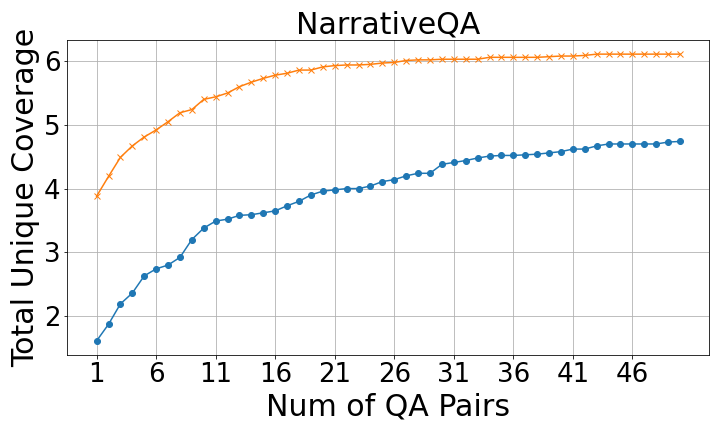
\includegraphics[width=\linewidth]{submissions/Tung2023/figs/NarrativeQA_Total Unique Coverage.png}
    % \caption{Total Unique Coverage in NarrativeQA}
    \label{fig:narrativeqa-total-unique-coverage}
\end{minipage}%
\begin{minipage}{0.33\textwidth}
    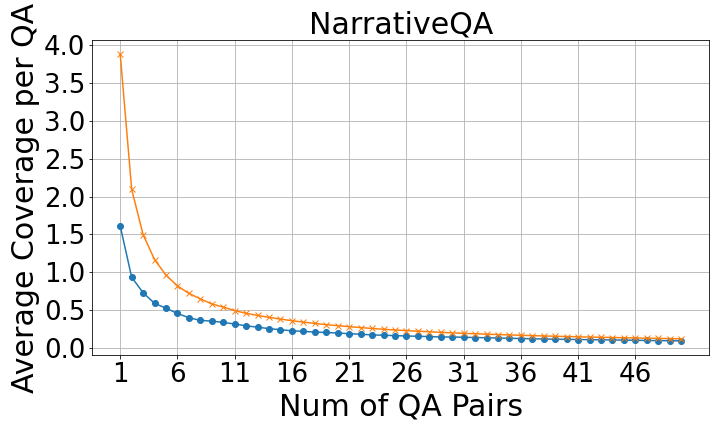
\includegraphics[width=\linewidth]{submissions/Tung2023/figs/NarrativeQA_Average Coverage per QA.png}
    \label{fig:narrativeqa-avg-cov-per-qa}
\end{minipage}%
\begin{minipage}{0.33\textwidth}
    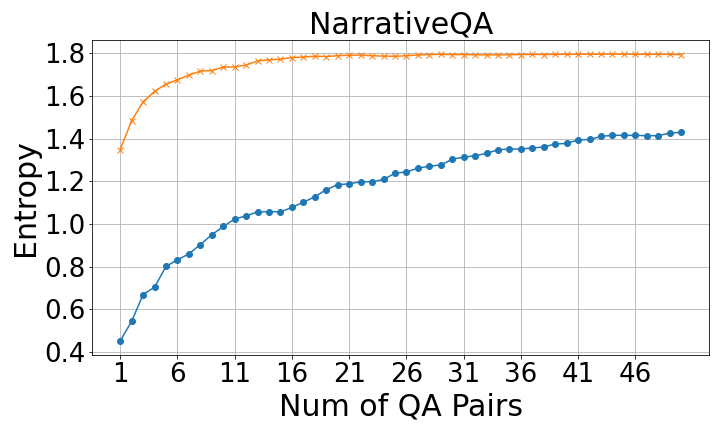
\includegraphics[width=\linewidth]{submissions/Tung2023/figs/NarrativeQA_Entropy.png}
    \label{fig:narrativeqa-entropy}
\end{minipage}

% Row for the SQuAD dataset
\noindent
\begin{minipage}{0.33\textwidth}
    \includegraphics[width=\linewidth]{submissions/Tung2023/figs/Squad_Total Unique Coverage.png}
    \label{fig:squad-total-unique-coverage}
\end{minipage}%
\begin{minipage}{0.33\textwidth}
    \includegraphics[width=\linewidth]{submissions/Tung2023/figs/Squad_Average Coverage per QA.png}
    \label{fig:squad-avg-cov-per-qa}
\end{minipage}%
\begin{minipage}{0.33\textwidth}
    \includegraphics[width=\linewidth]{submissions/Tung2023/figs/Squad_Entropy.png}
    \label{fig:squad-entropy}
\end{minipage}

% Row for the TriviaQA dataset
\noindent
\begin{minipage}{0.33\textwidth}
    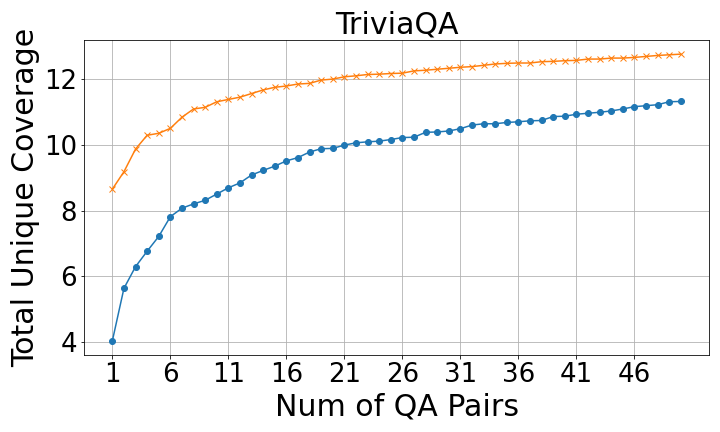
\includegraphics[width=\linewidth]{submissions/Tung2023/figs/TriviaQA_Total Unique Coverage.png}
    \label{fig:triviaqa-total-unique-coverage}
\end{minipage}%
\begin{minipage}{0.33\textwidth}
    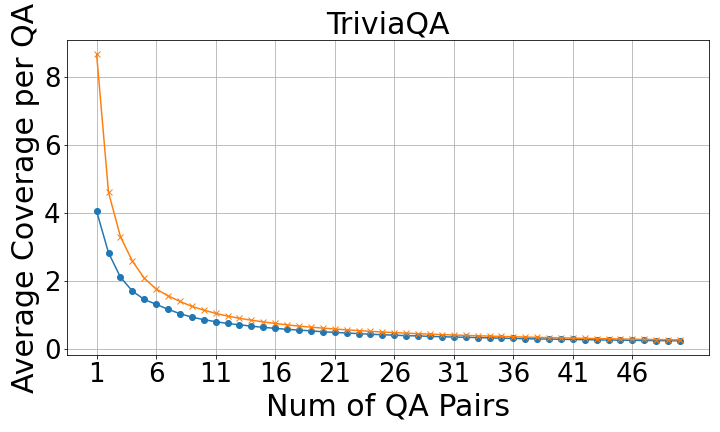
\includegraphics[width=\linewidth]{submissions/Tung2023/figs/TriviaQA_Average Coverage per QA.png}
    \label{fig:triviaqa-avg-cov-per-qa}
\end{minipage}%
\begin{minipage}{0.33\textwidth}
    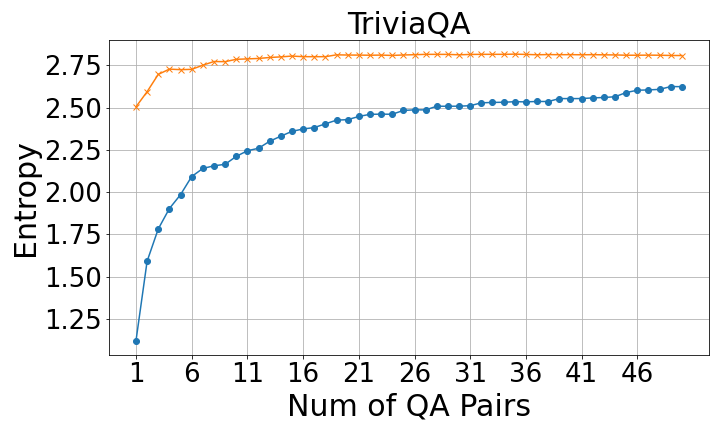
\includegraphics[width=\linewidth]{submissions/Tung2023/figs/TriviaQA_Entropy.png}
    \label{fig:triviaqa-entropy}
\end{minipage}


\begin{figure}[ht]
\centering
% Row for the Natural Questiondataset
\begin{minipage}{0.33\textwidth}
    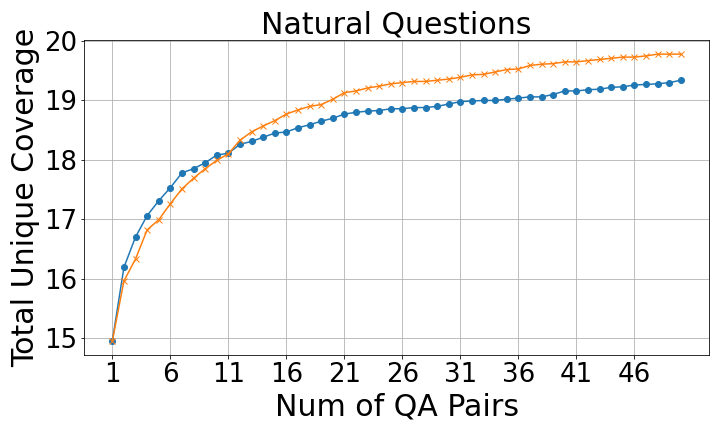
\includegraphics[width=\linewidth]{submissions/Tung2023/figs/Natural Questions_Total Unique Coverage.png}
    \label{fig:narrativeqa-total-unique-coverage}
\end{minipage}%
\begin{minipage}{0.33\textwidth}
    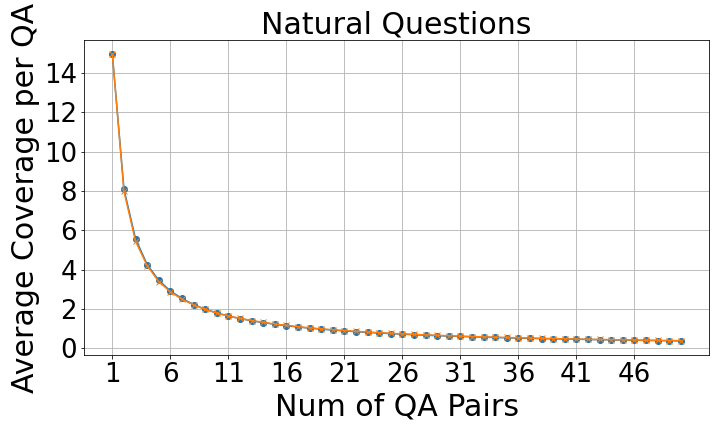
\includegraphics[width=\linewidth]{submissions/Tung2023/figs/Natural Questions_Average Coverage per QA.png}
    \label{fig:narrativeqa-avg-cov-per-qa}
\end{minipage}%
\begin{minipage}{0.33\textwidth}
    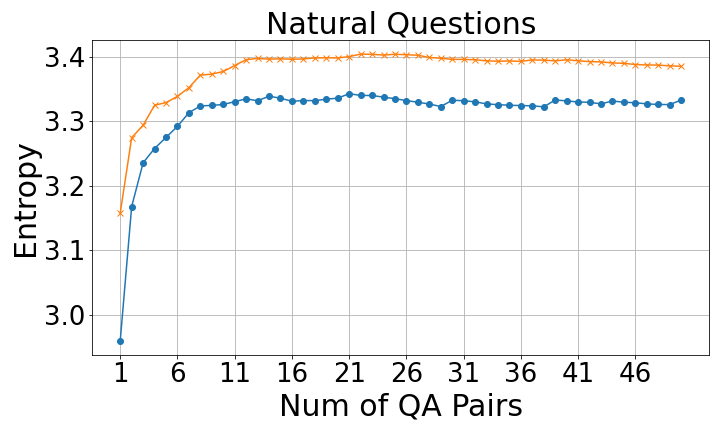
\includegraphics[width=\linewidth]{submissions/Tung2023/figs/Natural Questions_Entropy.png}
    \label{fig:narrativeqa-entropy}
\end{minipage}


\caption{Comparative analysis across datasets. The figure displays metrics for NarrativeQA, Squad, TriviaQA, and Natural Questions datasets, arranged row-wise. Columns represent Total Unique Coverage, Average Coverage per QA, and Entropy.}
\label{fig:dataset-comparisons}
\end{figure}

\fi

\begin{table}[H]
\caption{Comparison of Original, ReRanked, and Optimized Results Across Datasets. The table showcases metrics including Total Unique Coverage (TUC), Average Coverage per QA (ACPQ), and Entropy. Here, $\Delta$ denotes the improvement of optimized results compared to the original and re-ranked results.}
\label{tab:my-table}
\centering
\resizebox{!}{3.4cm}{%
\begin{tabular}{@{}llrrrrr@{}}
\toprule
Dataset                            & Metric           & Original & ReRanked & Optimized & $\Delta$Original (\%) & $\Delta$ReRanked (\%) \\ \midrule
\multirow{3}{*}{NarrativeQA}       & TUC & 2.52     & 5.25     & 6.89      & +173.66                & +31.26                 \\
                                   & ACPQ   & 1.38     & 2.43     & 2.87      & +107.52                & +18.38                 \\
                                   & ENTROPY          & 0.75     & 1.81     & 2.26      & +199.51                & +24.44                 \\ \midrule
\multirow{3}{*}{Squad}             & TUC & 2.71     & 4.62     & 5.63      & +108.15                & +21.97                 \\
                                   & ACPQ   & 1.38     & 2.53     & 2.87      & +108.33                & +13.05                 \\
                                   & ENTROPY          & 1.08     & 1.85     & 2.13      & +97.65                 & +14.59                 \\ \midrule
\multirow{3}{*}{TriviaQA}          & TUC & 7.65     & 11.40    & 14.28     & +86.65                 & +25.26                 \\
                                   & ACPA   & 1.91     & 2.94     & 3.56      & +86.18                 & +20.98                 \\
                                   & ENTROPY          & 2.08     & 2.96     & 3.36      & +61.62                 & +13.30                 \\ \midrule
\multirow{3}{*}{Natural Questions} & TUC & 18.03    & 17.80    & 21.55     & +19.50                 & +21.05                 \\
                                   & ACPQ   & 6.14     & 6.36     & 7.18      & +16.91                 & +12.98                 \\
                                   & ENTROPY          & 3.42     & 3.51     & 3.83      & +12.09                 & +9.11                  \\ \bottomrule
\end{tabular}%
}
\end{table}

\begin{figure}[h!]
    \centering
    
\includegraphics[width=0.45\textwidth]{submissions/Tung2023/figs/legend.png}\\%

% Row for the NarrativeQA dataset
    \begin{minipage}[h]{0.33\linewidth}
        \centering
        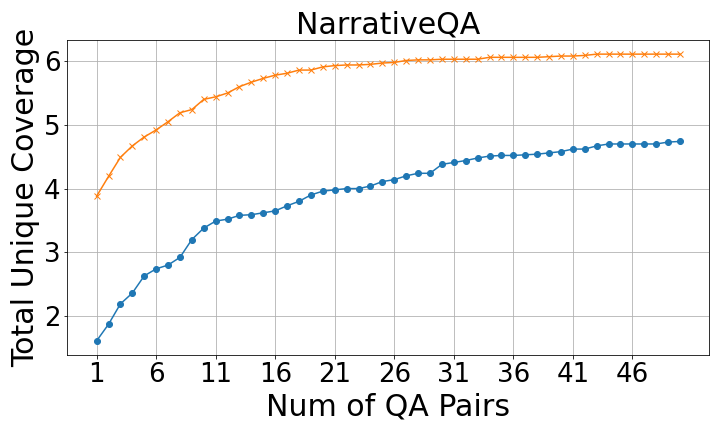
\includegraphics[width=\textwidth]{submissions/Tung2023/figs/NarrativeQA_Total Unique Coverage.png}
        % \subcaption{Total Unique Coverage for NarrativeQA}
    \label{fig:narrativeqa-total-unique-coverage}
    \end{minipage}
    \begin{minipage}[h]{0.33\linewidth}
        \centering
        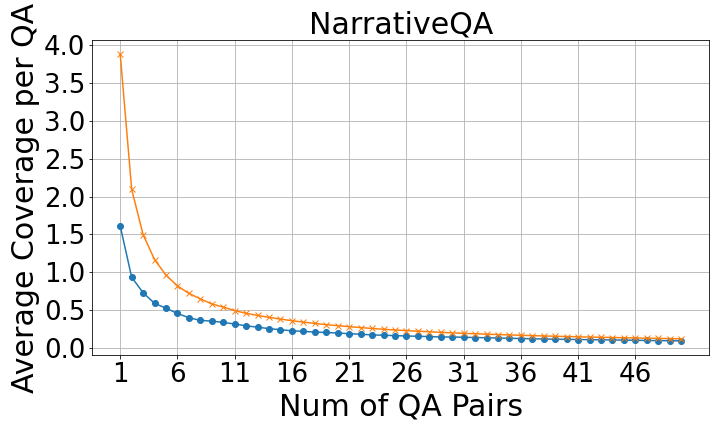
\includegraphics[width=\textwidth]{submissions/Tung2023/figs/NarrativeQA_Average Coverage per QA.png}
        %\subcaption{Attentive reader} 
    \label{fig:narrativeqa-avg-cov-per-qa}
    \end{minipage}
    \begin{minipage}[h]{0.33\linewidth}
        \centering
        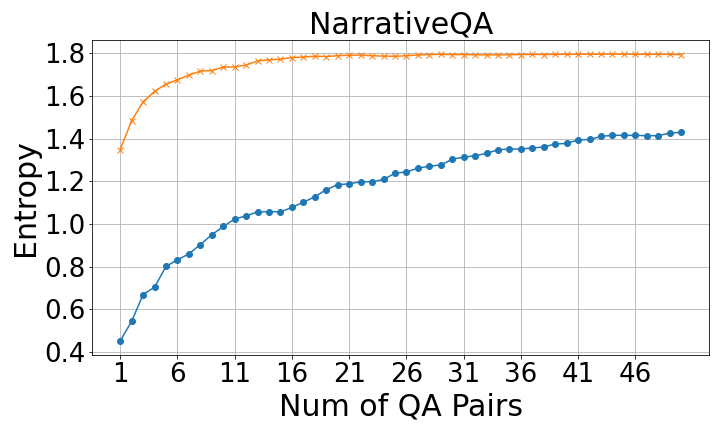
\includegraphics[width=\textwidth]{submissions/Tung2023/figs/NarrativeQA_Entropy.png}
        %\subcaption{Attentive reader} 
    \label{fig:narrativeqa-entropy}
    \end{minipage}
% Row for the SQuAD dataset
    \begin{minipage}[h]{0.33\linewidth}
        \centering
        \includegraphics[width=\textwidth]{submissions/Tung2023/figs/Squad_Total Unique Coverage.png}
        %\subcaption{Attentive reader} 
    \label{fig:squad-total-unique-coverage}
    \end{minipage}
    \begin{minipage}[h]{0.33\linewidth}
        \centering
        \includegraphics[width=\textwidth]{submissions/Tung2023/figs/Squad_Average Coverage per QA.png}
        %\subcaption{Attentive reader} 
    \label{fig:squad-avg-cov-per-qa}
    \end{minipage}
    \begin{minipage}[h]{0.33\linewidth}
        \centering
        \includegraphics[width=\textwidth]{submissions/Tung2023/figs/Squad_Entropy.png}
        %\subcaption{Attentive reader} 
    \label{fig:squad-entropy}
    \end{minipage}

% Row for the TriviaQA dataset
    \begin{minipage}[h]{0.33\linewidth}
        \centering
        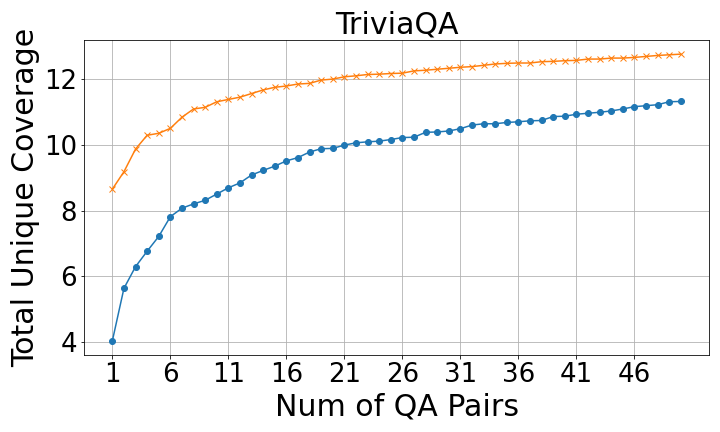
\includegraphics[width=\textwidth]{submissions/Tung2023/figs/TriviaQA_Total Unique Coverage.png}
        %\subcaption{Attentive reader} 
    \label{fig:triviaqa-total-unique-coverage}
    \end{minipage}
    \begin{minipage}[h]{0.33\linewidth}
        \centering
        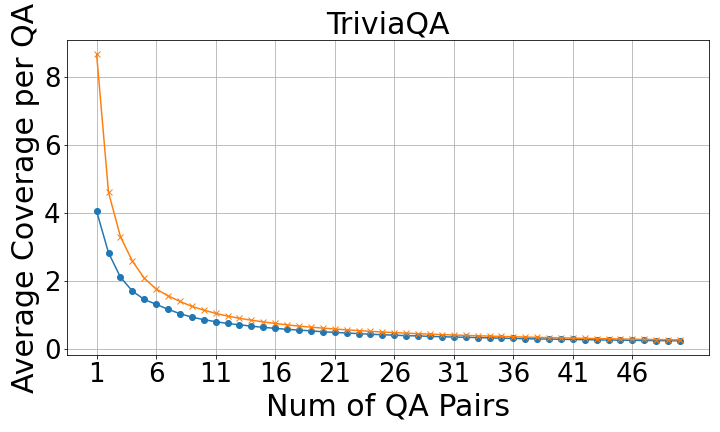
\includegraphics[width=\textwidth]{submissions/Tung2023/figs/TriviaQA_Average Coverage per QA.png}
        %\subcaption{Attentive reader} 
    \label{fig:triviaqa-avg-cov-per-qa}
    \end{minipage}
    \begin{minipage}[h]{0.33\linewidth}
        \centering
        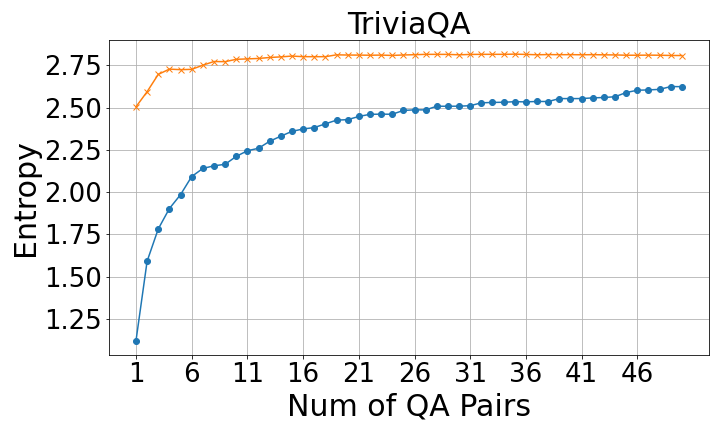
\includegraphics[width=\textwidth]{submissions/Tung2023/figs/TriviaQA_Entropy.png}
        %\subcaption{Attentive reader} 
    \label{fig:triviaqa-entropy}
    \end{minipage}

% Row for the Natural Questions datasett
    \begin{minipage}[h]{0.33\linewidth}
        \centering
        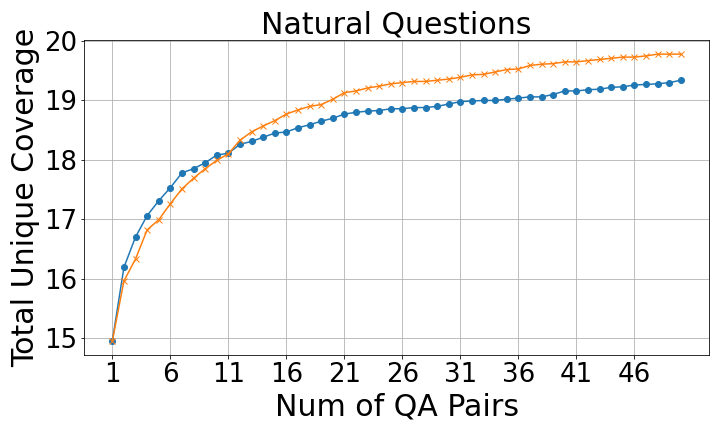
\includegraphics[width=\textwidth]{submissions/Tung2023/figs/Natural Questions_Total Unique Coverage.png}
        %\subcaption{Attentive reader} 
    \label{fig:narrativeqa-total-unique-coverage}
    \end{minipage}
    \begin{minipage}[h]{0.33\linewidth}
        \centering
        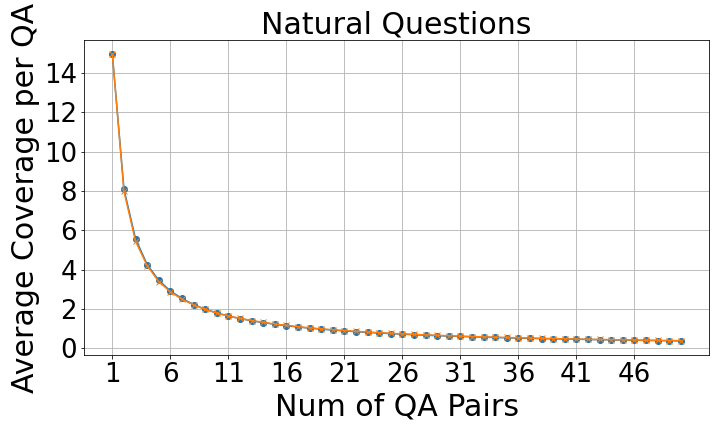
\includegraphics[width=\textwidth]{submissions/Tung2023/figs/Natural Questions_Average Coverage per QA.png}
        %\subcaption{Attentive reader} 
    \label{fig:narrativeqa-avg-cov-per-qa}
    \end{minipage}
    \begin{minipage}[h]{0.33\linewidth}
        \centering
        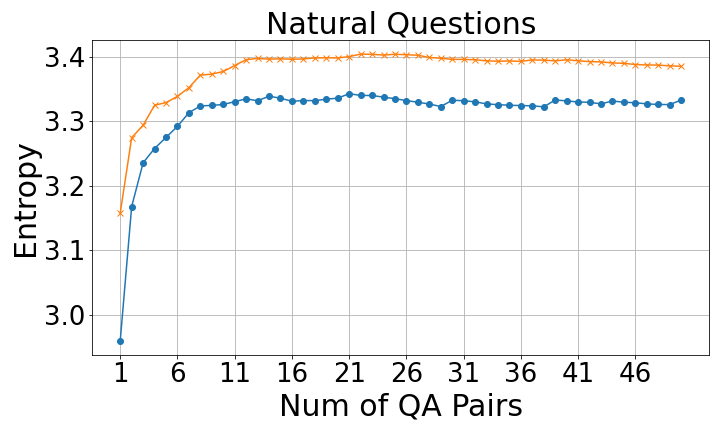
\includegraphics[width=\textwidth]{submissions/Tung2023/figs/Natural Questions_Entropy.png}
        %\subcaption{Attentive reader} 
    \label{fig:narrativeqa-entropy}
    \end{minipage}
 
\caption{Coverage and Diversity Comparison}
\label{fig:dataset-comparisons}
\end{figure}



The results of diversity and coverage comparison, illustrated in the Fig\ref{fig:dataset-comparisons}, distinctly showcase the efficacy of our re-ranking method in enhancing the novelty aspect of interestingness. Across various datasets, the re-ranked sets consistently outperform the original ones in Total Unique Context Entity Coverage and Average Context Entity Coverage per QA, indicating a broader and more diverse range of context entities being addressed. While the Entropy metric remains stable, suggesting a balanced distribution of entities, the overall increase in coverage metrics confirms that our approach successfully selects more novel question-answer pairs, aligning with our objective of providing novel contents in text enrichment tasks.


The comparative analysis of the results pre- and post-subgraph optimization is presented in Table \ref{tab:my-table}. It is evident that the performance significantly improves with the optimized results compared to the original outcomes derived from direct dense retrieval, and it also surpasses the direct reranked results based on our path analysis. This substantiates the effectiveness of our optimization method in procuring a set of QA pairs that is not only diverse but also offers an enhanced collective quality over focusing solely on individual pairs.

% \begin{table}[]
%     \centering
%     \begin{tabular}{llrrrrr}
%     \toprule
%            Dataset &            Metric &  Original &  ReRanked &  Optimized &  $\Delta$Original (\%) &  $\Delta$ReRanked (\%) \\
%     \midrule
%        NarrativeQA &  total unique cov &      2.52 &      5.25 &       6.89 &                         +173.66 &                          +31.26 \\
%        NarrativeQA &    avg cov per qa &      1.38 &      2.43 &       2.87 &                         +107.52 &                          +18.38 \\
%        NarrativeQA &           entropy &      0.75 &      1.81 &       2.26 &                         +199.51 &                          +24.44 \\
%              Squad &  total unique cov &      2.71 &      4.62 &       5.63 &                         +108.15 &                          +21.97 \\
%              Squad &    avg cov per qa &      1.38 &      2.53 &       2.87 &                         +108.33 &                          +13.05 \\
%              Squad &           entropy &      1.08 &      1.85 &       2.13 &                          97.65 &                          +14.59 \\
%           TriviaQA &  total unique cov &      7.65 &     11.40 &      14.28 &                          +86.65 &                          +25.26 \\
%           TriviaQA &    avg cov per qa &      1.91 &      2.94 &       3.56 &                          +86.18 &                          +20.98 \\
%           TriviaQA &           entropy &      2.08 &      2.96 &       3.36 &                          +61.62 &                          +13.30 \\
%  Natural Questions &  total unique cov &     18.03 &     17.80 &      21.55 &                          +19.50 &                          21.05 \\
%  Natural Questions &    avg cov per qa &      6.14 &      6.36 &       7.18 &                          +16.91 &                          +12.98 \\
%  Natural Questions &           entropy &      3.42 &      3.51 &       3.83 &                          +12.09 &                           +9.11 \\
% \bottomrule
% \end{tabular}
%     \caption{Caption}
%     \label{tab:my_label}
% \end{table}



% \begin{table}[H]
% \caption{Comparison of Original, ReRanked, and Optimized Results Across Datasets. The table showcases metrics including Total Unique Coverage (TUC), Average Coverage per QA (ACPQ), and Entropy. Here, $\Delta$ denotes the improvement of optimized results compared to the original and re-ranked results.}
% \label{tab:my-table}
% \resizebox{\textwidth}{!}{%
% \begin{tabular}{@{}llrrrrr@{}}
% \toprule
% Dataset                            & Metric           & Original & ReRanked & Optimized & $\Delta$Original (\%) & $\Delta$ReRanked (\%) \\ \midrule
% \multirow{3}{*}{NarrativeQA}       & TUC & 2.52     & 5.25     & 6.89      & +173.66                & +31.26                 \\
%                                    & ACPQ   & 1.38     & 2.43     & 2.87      & +107.52                & +18.38                 \\
%                                    & ENTROPY          & 0.75     & 1.81     & 2.26      & +199.51                & +24.44                 \\ \midrule
% \multirow{3}{*}{Squad}             & TUC & 2.71     & 4.62     & 5.63      & +108.15                & +21.97                 \\
%                                    & ACPQ   & 1.38     & 2.53     & 2.87      & +108.33                & +13.05                 \\
%                                    & ENTROPY          & 1.08     & 1.85     & 2.13      & +97.65                 & +14.59                 \\ \midrule
% \multirow{3}{*}{TriviaQA}          & TUC & 7.65     & 11.40    & 14.28     & +86.65                 & +25.26                 \\
%                                    & ACPA   & 1.91     & 2.94     & 3.56      & +86.18                 & +20.98                 \\
%                                    & ENTROPY          & 2.08     & 2.96     & 3.36      & +61.62                 & +13.30                 \\ \midrule
% \multirow{3}{*}{Natural Questions} & TUC & 18.03    & 17.80    & 21.55     & +19.50                 & +21.05                 \\
%                                    & ACPQ   & 6.14     & 6.36     & 7.18      & +16.91                 & +12.98                 \\
%                                    & ENTROPY          & 3.42     & 3.51     & 3.83      & +12.09                 & +9.11                  \\ \bottomrule
% \end{tabular}%
% }
% \end{table}


\subsection{Assessing the Impact of Re-ranking on Superficial QA Reduction}
\label{exp:2}
% This experiment is designed to evaluate the effectiveness of our approach in modeling the complexity aspect of interestingness. We utilize Algo.\ref{alg:refined_graph_path_analysis}, which assigns scores to each question-answer (QA) pair based on specific criteria derived from the path analysis. These scores are then used to re-rank the QAs initially retrieved by a standard dense retrieval framework. The underlying premise of our algorithm is its focus on complexity and novelty within the interestingness model. Consequently, we hypothesize that re-ranking QAs based on these scores will lead to a reduction in the proportion of superficial QAs among the top results. To test our hypothesis, we compare the superficial QA distribution in both the original retrieval and the re-ranked list, observing whether the re-ranking reduces superficial content in the top results. 

This experiment aims to assess our approach's effectiveness in capturing the complexity aspect of interestingness. Utilizing Algo.\ref{alg:refined_graph_path_analysis}, we assign scores to QA pairs based on criteria from path analysis, then re-rank QAs initially retrieved by a standard dense retrieval framework. We hypothesize that our approach, which enhances complexity and novelty, will reduce the prevalence of superficial QAs in the top results. This hypothesis will be tested by comparing the superficial QA distribution in both the original and re-ranked lists.

% This approach focuses on enhancing complexity and novelty within our interestingness model. We hypothesize that this re-ranking will decrease the presence of superficial QAs in the top results and plan to test this by comparing the distribution of such QAs in the original and re-ranked lists.

We employ the Natural Questions dataset \cite{DBLP:journals/tacl/KwiatkowskiPRCP19} for its categorization of short-answer questions, often considered superficial compared to the complex and deep `interestingness' QAs our research targets. Our evaluation metric is the percentage of superficial QAs in the top $n$ results, where a QA is labeled superficial if it's answerable with a short response, which is usually one or two words.

\begin{figure}[h]
  \centering
  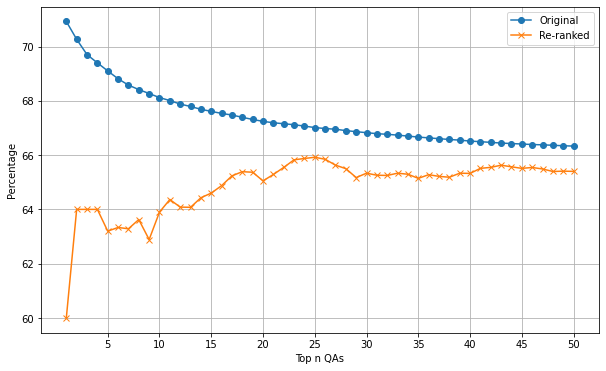
\includegraphics[width=0.65\textwidth]{submissions/Tung2023/figs/sup_re.png}
  \caption{Percentage of Superficial QAs in Natural Questions}
  \label{fig:superficial_qas}
\end{figure}

% Results and Discussion
The results, depicted in Fig.\ref{fig:superficial_qas}, demonstrate a notable decrease, more than $10\%$ at the beginning, in the prevalence of superficial QA pairs within the re-ranked results, with the re-ranking line consistently positioned below that of the original. This trend indicates that our path analysis algorithm has effectively prioritized QAs of greater complexity. Initially, the original results exhibit a high percentage of superficial QAs, aligning with findings from \cite{sciavolino2021simple}. The tendency to favor frequently occurring entities often results in the initial selection of less complex QA pairs. As $n$ increases, the percentage of superficial QAs in the re-ranked results gradually rises, while it decreases in the original dense retrieval results. This pattern can be attributed to the limited availability of non-superficial QAs in certain contexts, exemplified by the `Harry Potter' case discussed in Sec.\ref{sec:intro}.


% \input{./chapter6.conclusion.tex}
\section{Conclusion}

In this study, we tackled the challenge of enhancing text enrichment using QA datasets like Natural Questions and SQuAD through an innovative approach involving the creation of an extensive entity co-occurrence graph, from which context-specific subgraphs were derived. This led to a rule-based path analysis and a novel scoring system, assessing each QA pair's relevance and engagement value, thus enriching the reader's experience. Additionally, our framework discusses aspects of personal data management and personalization, suggesting ways to align personalized content with individual privacy needs. Our methodology's effectiveness was evident in two key experiments: Experiment \ref{exp:1} highlighted our re-ranking method's ability to enhance novelty, as shown by improved coverage metrics, and Experiment \ref{exp:2} demonstrated a significant reduction in superficial QAs, emphasizing the prioritization of more complex, contextually relevant content. These results underscore our approach's potential to fill knowledge gaps and captivate readers, marking a significant step forward in text enrichment using QA datasets. 

\section{Acknowledgments}
%The authors would like to thank the anonymous reviewers for insightful comments and helpful suggestions.
%\small{This research is supported by the National Research Foundation, Singapore under its Strategic Capability Research Centres Funding Initiative. Any opinions, findings and conclusions or recommendations expressed in this material are those of the author(s) and do not reflect the views of National Research Foundation, Singapore.\\
%This research/project is supported by the Ministry of Education, Singapore, under its MOE AcRF TIER 3 Grant (MOE-MOET32022-0001). Any opinions, findings and conclusions or recommendations expressed in this material are those of the author(s) and do not reflect the views of the Ministry of Education, Singapore.
%}

\small{This research is supported by the National Research Foundation, Singapore under its Strategic Capability Research Centres Funding Initiative and the Ministry of Education, Singapore, under its MOE AcRF TIER 3 Grant (MOE-MOET32022-0001).
Any opinions, findings and conclusions or recommendations expressed in this material are those of the author(s) and do not reflect the views of National Research Foundation, Singapore and the Ministry of Education, Singapore.}


\begin{thebibliography}{10}

\bibitem{berlyne1960conflict}
Daniel~E Berlyne.
\newblock Conflict, arousal, and curiosity.
\newblock 1960.

\bibitem{berlyne1974studies}
Daniel~E Berlyne.
\newblock {\em Studies in the new experimental aesthetics: Steps toward an objective psychology of aesthetic appreciation.}
\newblock Hemisphere, 1974.

\bibitem{bolton1910attention}
Frederick~E Bolton.
\newblock Attention and interest: A study in psychology and education.
\newblock {\em The Journal of Philosophy, Psychology and Scientific Methods}, 7(17):474--475, 1910.

\bibitem{DBLP:conf/acl/ChenFWB17}
Danqi Chen, Adam Fisch, Jason Weston, and Antoine Bordes.
\newblock Reading wikipedia to answer open-domain questions.
\newblock In {\em {ACL} {(1)}}, pages 1870--1879. Association for Computational Linguistics, 2017.

\bibitem{DBLP:conf/acl/GardnerC18}
Christopher Clark and Matt Gardner.
\newblock Simple and effective multi-paragraph reading comprehension.
\newblock In {\em {ACL} {(1)}}, pages 845--855. Association for Computational Linguistics, 2018.

\bibitem{DBLP:conf/iclr/DasDZM19}
Rajarshi Das, Shehzaad Dhuliawala, Manzil Zaheer, and Andrew McCallum.
\newblock Multi-step retriever-reader interaction for scalable open-domain question answering.
\newblock In {\em {ICLR} (Poster)}. OpenReview.net, 2019.

\bibitem{DBLP:conf/aaai/FatmaCS17}
Nausheen Fatma, Manoj~Kumar Chinnakotla, and Manish Shrivastava.
\newblock The unusual suspects: Deep learning based mining of interesting entity trivia from knowledge graphs.
\newblock In {\em {AAAI}}, pages 1107--1113. {AAAI} Press, 2017.

\bibitem{fredrickson1998good}
Barbara~L Fredrickson.
\newblock What good are positive emotions?
\newblock {\em Review of general psychology}, 2(3):300--319, 1998.

\bibitem{izard2000motivational}
Carroll~E Izard and Brian~P Ackerman.
\newblock Motivational, organizational, and regulatory functions of discrete emotions.
\newblock {\em Handbook of emotions}, 2:253--264, 2000.

\bibitem{DBLP:conf/acl/JoshiCWZ17}
Mandar Joshi, Eunsol Choi, Daniel~S. Weld, and Luke Zettlemoyer.
\newblock Triviaqa: {A} large scale distantly supervised challenge dataset for reading comprehension.
\newblock In {\em {ACL} {(1)}}, pages 1601--1611. Association for Computational Linguistics, 2017.

\bibitem{DBLP:conf/eacl/KamigaitoKSO21}
Hidetaka Kamigaito, Jingun Kwon, Young{-}In Song, and Manabu Okumura.
\newblock A new surprise measure for extracting interesting relationships between persons.
\newblock In {\em {EACL} (System Demonstrations)}, pages 231--237. Association for Computational Linguistics, 2021.

\bibitem{DBLP:conf/emnlp/KarpukhinOMLWEC20}
Vladimir Karpukhin, Barlas Oguz, Sewon Min, Patrick S.~H. Lewis, Ledell Wu, Sergey Edunov, Danqi Chen, and Wen{-}tau Yih.
\newblock Dense passage retrieval for open-domain question answering.
\newblock In {\em {EMNLP} {(1)}}, pages 6769--6781. Association for Computational Linguistics, 2020.

\bibitem{DBLP:journals/tacl/KociskySBDHMG18}
Tom{\'{a}}s Kocisk{\'{y}}, Jonathan Schwarz, Phil Blunsom, Chris Dyer, Karl~Moritz Hermann, G{\'{a}}bor Melis, and Edward Grefenstette.
\newblock The narrativeqa reading comprehension challenge.
\newblock {\em Trans. Assoc. Comput. Linguistics}, 6:317--328, 2018.

\bibitem{krapp1999interest}
Andreas Krapp.
\newblock Interest, motivation and learning: An educational-psychological perspective.
\newblock {\em European journal of psychology of education}, 14:23--40, 1999.

\bibitem{DBLP:journals/tacl/KwiatkowskiPRCP19}
Tom Kwiatkowski, Jennimaria Palomaki, Olivia Redfield, Michael Collins, Ankur~P. Parikh, Chris Alberti, Danielle Epstein, Illia Polosukhin, Jacob Devlin, Kenton Lee, Kristina Toutanova, Llion Jones, Matthew Kelcey, Ming{-}Wei Chang, Andrew~M. Dai, Jakob Uszkoreit, Quoc Le, and Slav Petrov.
\newblock Natural questions: a benchmark for question answering research.
\newblock {\em Trans. Assoc. Comput. Linguistics}, 7:452--466, 2019.

\bibitem{DBLP:conf/emnlp/MaPMC00G21}
Nianzu Ma, Alexander Politowicz, Sahisnu Mazumder, Jiahua Chen, Bing Liu, Eric Robertson, and Scott Grigsby.
\newblock Semantic novelty detection in natural language descriptions.
\newblock In {\em {EMNLP} {(1)}}, pages 866--882. Association for Computational Linguistics, 2021.

\bibitem{DBLP:conf/ijcai/PrakashCPG15}
Abhay Prakash, Manoj~Kumar Chinnakotla, Dhaval Patel, and Puneet Garg.
\newblock Did you know? - mining interesting trivia for entities from wikipedia.
\newblock In {\em {IJCAI}}, pages 3164--3170. {AAAI} Press, 2015.

\bibitem{DBLP:conf/emnlp/RajpurkarZLL16}
Pranav Rajpurkar, Jian Zhang, Konstantin Lopyrev, and Percy Liang.
\newblock Squad: 100, 000+ questions for machine comprehension of text.
\newblock In {\em {EMNLP}}, pages 2383--2392. The Association for Computational Linguistics, 2016.

\bibitem{schraw2001situational}
Gregory Schraw and Stephen Lehman.
\newblock Situational interest: A review of the literature and directions for future research.
\newblock {\em Educational psychology review}, 13:23--52, 2001.

\bibitem{sciavolino2021simple}
Christopher Sciavolino, Zexuan Zhong, Jinhyuk Lee, and Danqi Chen.
\newblock Simple entity-centric questions challenge dense retrievers.
\newblock {\em arXiv preprint arXiv:2109.08535}, 2021.

\bibitem{DBLP:journals/corr/abs-1906-05807}
Min~Joon Seo, Jinhyuk Lee, Tom Kwiatkowski, Ankur~P. Parikh, Ali Farhadi, and Hannaneh Hajishirzi.
\newblock Real-time open-domain question answering with dense-sparse phrase index.
\newblock {\em CoRR}, abs/1906.05807, 2019.

\bibitem{silvia2005interesting}
Paul~J Silvia.
\newblock What is interesting? exploring the appraisal structure of interest.
\newblock {\em Emotion}, 5(1):89, 2005.

\bibitem{DBLP:conf/cikm/TangHLTWYZ17}
Yixuan Tang, Weilong Huang, Qi~Liu, Anthony K.~H. Tung, Xiaoli Wang, Jisong Yang, and Beibei Zhang.
\newblock Qalink: Enriching text documents with relevant q{\&}a site contents.
\newblock In {\em {CIKM}}, pages 1359--1368. {ACM}, 2017.

\bibitem{tomkins1962affect}
Silvan Tomkins.
\newblock {\em Affect imagery consciousness: Volume I: The positive affects}.
\newblock Springer publishing company, 1962.

\bibitem{DBLP:conf/wsdm/TsurelPGS17}
David Tsurel, Dan Pelleg, Ido Guy, and Dafna Shahaf.
\newblock Fun facts: Automatic trivia fact extraction from wikipedia.
\newblock In {\em {WSDM}}, pages 345--354. {ACM}, 2017.

\end{thebibliography}



\end{document}


